\chapter{Fit model and Results}
\label{ch:results}

% **************************** Define Graphics Path **************************
\ifpdf
    \graphicspath{{Chapter7/Figs/Raster/}{Chapter7/Figs/PDF/}{Chapter7/Figs/}}
\else
    \graphicspath{{Chapter7/Figs/Vector/}{Chapter7/Figs/}}
\fi


%********************************** % First Section  *************************************
\section{Likelihood Model}  %Section - 1.1 
\label{sec:results_likelihood}
The likelihood is defined for each analysis category of \nb and \nj as follows.

\subsection{Hadronic Signal Region}

Let $n^i$ be the observed number of events 
following the full selection in the $i^{th}$ of $N$ bins of \HT. The likelihood
is constructed as:
% 
\begin{equation}
L_{hadronic} = \prod_i \text{Pois}(n^i | b^i + s^i),
\end{equation}
% 
where $b^i$ and $s^i$ represent the expected number of background events from SM 
processes and the expected number of signal events in the bin $i$. Pois is 
the Poisson distribution:

\begin{equation}
Pois(k;\lambda) = \frac{1}{k!}\lambda^k e^{-\lambda}.
\end{equation}


\subsection{Electroweak Background Contribution}
The background is considered to be entirely EWK in origin ($b^i = \text{EWK}^i$), as QCD
is made negligible, so can be de-constructed using the relative fraction
of \zinv events, \fzinv as:
% 
\begin{equation}
\text{Z}_{inv}^i = \fzinv \times \text{EWK}^i,
\label{eq:ewk_frac_z}
\end{equation}
\begin{equation}
\text{ttW}^i = (1-\fzinv) \times \text{EWK}^i,
\label{eq:ewk_frac_ttw}
\end{equation}
% 
where $\text{EWK}^i$ is number of expected events from the total EWK background,
$\text{Z}_{\text{inv}}^i$ is the number of expected events from the \zinv 
contribution and $\text{ttW}^i$ is the number of expect events from the W boson 
production and top quark decay contribution, all in the $i^{th}$ bin. The variable 
\fzinv is allowed to float between 0 and 1.

EWK backgrounds are predicted using sideband control regions and transfer 
factors (chapter~\ref{ch:background}). Let $n_{\gamma}^i$, $n_{\mu}^i$ and
$n_{\mu\mu}^i$ be
the observed event counts in the \gj, \mj and \mmj control regions, 
respectively, with corresponding yields in MC: \mcp, \mcm, \mcmm. These are
further separated into contributions from \zinv, \mczinv, and \text{ttW},
\mcttw. Purely as an arbitrary convention, transfer factors are defined as
the inverse as those of the analysis:
% 
\begin{equation}
r_{\gamma}^i = \frac{\mcp}{\mczinv};\;\;\;
r_{\mu\mu}^i = \frac{\mcmm}{\mczinv};\;\;\;
r_{\mu}^i = \frac{\mcm}{\mcttw},
\end{equation}
% 
and so likelihoods are written as:
% 
\begin{equation}
L_{\gamma} = \prod_i \text{Pois}(n_{\gamma}^i | \rhopz \cdot r^i_{\gamma} \cdot \text{Z}^i_{\text{inv}}),
\label{eq:lterm_pho}
\end{equation}
\begin{equation}
L_{\mu\mu} = \prod_i \text{Pois}(n_{\mu\mu}^i | \rhommz \cdot r^i_{\mu\mu} \cdot \text{Z}^i_{\text{inv}}),
\label{eq:lterm_mumu}
\end{equation}
\begin{equation}
L_{\mu} = \prod_i \text{Pois}(n_{\mu}^i | \rhomw \cdot r^i_{\mu} \cdot \text{ttW}^i + s_{\mu}^i).
\label{eq:lterm_mu}
\end{equation}
% 
Both equations~\ref{eq:lterm_pho} and \ref{eq:lterm_mumu} are used to estimate the 
maximum likelihood value for $Z^i_{\text{inv}}$, alongside Equation~\ref{eq:lterm_mu} 
for $ttW^i$, all considered simultaneously through the relationships defined in
equations~\ref{eq:ewk_frac_z} and \ref{eq:ewk_frac_ttw}.

The terms \rhopz, \rhommz and \rhomw are correction factors accommodating the
systematic uncertainties associated with the control region based background 
predictions. The relative uncertainties are derived in
Section~\ref{sec:background_systematics} and represented by the terms \sigmapz, \sigmammz
and \sigmamw, their 
values summarised in Table~\ref{tab:syst_values}. Systematics enter the total
likelihood as:
% 
\begin{equation}
L_{\gamma\text{ syst.}} = \prod_j \text{Logn}(1.0 | \rhopz, \sigmapz),
\end{equation}
\begin{equation}
L_{\mu\mu\text{ syst.}} = \prod_j \text{Logn}(1.0 | \rhommz, \sigmammz),
\end{equation}
\begin{equation}
L_{\mu\text{ syst.}} = \prod_j \text{Logn}(1.0 | \rhomw, \sigmamw),
\end{equation}
% 
where Logn is the log-normal distribution (as recommended by~\cite{cousins-log-normal}):
% 
\begin{equation}
\text{Logn}(x|\mu, \sigma) = \frac{1}{x\sqrt{2\pi}\text{ln}k} exp \Bigg(-\frac{\text{ln}^2 \big(\frac{x}{\mu}\big)}{2\text{ln}^2k}\Bigg); \xspace k = 1+\sigma .
\end{equation}
% 
These terms are combined as:
% 
\begin{equation}
L_{EWK\text{ syst.}} = L_{\gamma\text{ syst.}} \times L_{\mu\mu\text{ syst.}} \times L_{\mu\text{ syst.}}.
\end{equation}
% 
For $\nb \geq 2$ categories, the \mj control region is used to predict \zinv and
\ttw combined, giving:
% 
\begin{equation}
{r'}^i_{\mu} = \frac{\mcm}{MC^i_{\ttbar + W + \text{Z}_{\text{inv}}}};
\end{equation}
% 
\begin{equation}
L_{\mu} = \prod_i \text{Pois}(n_{\mu}^i | \rhomw \cdot {r'}_{\mu}^i \cdot \text{EWK}^i + s_{\mu}^i).
\end{equation}
% 
Terms corresponding to the \mmj and \gj regions are subsequently dropped.

\subsection{Signal Contribution}

Let $x$ be the cross section of the signal model under test, which can be varied
according to a multiplicative factor $f$ (a.k.a. the ``mu-factor''), and $l$ be 
the luminosity of the relevant collected data sample. $\epsilon^i_{had}$ and
$\epsilon^i_{\mu}$ are the signal acceptances of the hadronic and muon 
selections, respectively, for the given signal model. Finally, let $\delta$ be 
the relative systematic uncertainty on that signal acceptance, and $\rho_{sig}$ 
be the corrective factor to the signal yield floated to accommodate this uncertainty. 
Therefore the yield of signal events for the hadronic region, $s^i$, and the 
yield of signal events in the muon region (i.e. ``signal contamination''),
$s^i_{\mu}$, can be written as:
% 
\begin{equation}
s^i = f\rho_{sig}xl\epsilon_{had} , 
\end{equation}
\begin{equation}
s^i_{\mu} = f\rho_{sig}xl\epsilon_{\mu} .
\end{equation}
% 
Furthermore, the signal systematic contribution to the likelihood is included as
the term:
% 
\begin{equation}
L_{signal} = \text{Logn}(1.0 | \rho_{sig}, \delta) .
\end{equation}
% 
\subsection{Total Likelihood}

For a given analysis category $k$ (\nb, \nj), the total likelihood is 
constructed as:
% 
\begin{equation}
L^k_{total} = L^k_{hadronic} \times L^k_{\mu} \times L^k_{\gamma} \times L^k_{\mu\mu} 
\times L^k_{\text{EWK syst.}} .
\label{eq:total_likelihood}
\end{equation}
% 
The number of nuisance parameters varies between different analysis categories, 
dependent on the number of \HT bins and control regions, as summarised in
Table~\ref{tab:nuisance_param_summary}.

\begin{table}[ht!]
  \caption{Summary of likelihood nuisance parameters.}
  \label{tab:nuisance_param_summary}
  \centering
  \footnotesize
  \begin{tabular}{ lll }
    \hline
    \hline
    Description                             & Categories    & Nuisance Parameters \\ [1.0ex]
    \hline
    \multirow{2}{*}{11 \HT bins, ($\mu, \mu\mu, \gamma$)}    & \multirow{2}{*}{\njlow/\njhigh, \nb = 0, 1}&
    $\{\text{EWK}^i, \fzinv\}_{i=0}^{10}, \{ \rhopz \}_{i=3}^{6},$\\
    && $\{ \rhommz, \rhomw \}_{i=0}^{6}$  \\
    8 \HT bins, ($\mu$)                     & \njlow/\njhigh, \nb = 2, 3, $\geq$4    & $\{\text{EWK}^i, \fzinv\}_{i=0}^{
    8}, \{\rhomwz \}_{i=0}^{6}$  \\
    3 \HT bins, ($\mu$)                     & \njlow/\njhigh, \nb = 2, 3, $\geq$4    & $\{\text{EWK}^i\}_{i=0}^{3},
    \{\rhomwz \}_{i=0}$\\
    \hline
    \hline
  \end{tabular}
\end{table}

When considering signal an additional term is introduced:
% 
\begin{equation}
L = L_{signal} \times \prod_k L^k_{total} .
\label{eq:total_likelihood_wsignal}
\end{equation}
% 
% \subsection{Notes on syst modelling}
% lognormal instead of gaussian PDF - these are used for systematics modelling.

% see:
% \verb!http://www.physics.ucla.edu/~cousins/stats/cousins_lognormal_prior.pdf!

% if you had a parameter with mean of 0.3 and variance of 0.1, you could have a 
% distro which would give you negative values of your PDF, if you used gaussian. 
% therefore we use lognormal.

% The lognormal distribution has three variables as input. $Logn(x|\rho, \sigma)$

% \begin{description}
% \item[$\sigma$ parameter]\hfill \\ this is similar to the width, if it were a gaussian 
% distribution. It is essentially the derived systematic error as taken from the 
% closure tests (I think...!). The smaller the value, the more the $\rho$ 
% parameters may need to be pulled in order to make the fit.
% \item[$\rho$ parameter] \hfill \\ the mean of the syst error. this is a parameter
% (nuisance?) which is allowed to float in the fit. It essentially represents how 
% much you have to pull on your systematics in order for the observations to match
% the background predictions. If it's pulled a lot (many sigma away from 1.) then 
% your observations really don't fit your predictions, or you've really 
% underestimated your systematics! Large deviations from 1 (in terms of the
% $\sigma$ parameter) indicate an unhealthy fit...
% \end{description}



%********************************** % Second Section  *************************************
\section{Fit Results}  %Section - 1.2
\label{sec:results_fit}
The likelihood model described in Section~\ref{sec:results_likelihood} is used
to relate the observations in the signal and control regions, accommodate the
calculated background systematic uncertainties, and allow for the presence of
any potential signal. In order to test the compatibility with a Standard
Model only hypothesis, signal contribution is set to zero and the likelihood is
maximized over all parameters using \ROOFIT~\cite{roofit} and
\MINUIT~\cite{James:1975dr}, for each analysis category of \nb and \nj.

Uncertainties are determined by performing a number of pseudo-experiments for
each (\nb, \nj) category and \HT bin, with the fit yields being entered into a
histogram, using the 68~\% quantiles as the fit uncertainties.

Two different procedures are used to determine fits to observations, as described
in the following sections.

\subsection{Fit without Signal region}
\label{sec:results_fit_green}
An ``a priori'' fit is made by considering only yields from the control regions,
and not data observations in the hadronic signal region. The results of this fit
are shown in Figures~\ref{fig:green_fits_0b_le3j}, \ref{fig:green_fits_1b_le3j}, \ref{fig:green_fits_2b_le3j}, \ref{fig:green_fits_0b_ge4j}, \ref{fig:green_fits_1b_ge4j}, \ref{fig:green_fits_2b_ge4j}, \ref{fig:green_fits_3b_ge4j} and \ref{fig:green_fits_ge4b_ge4j},
and summarised in Table~\ref{tab:ensemble-summary-priori}. As data
observations from the signal region are not considered, it should be noted that
the `EWK Prediction' is simply the result of the transfer factor method
(described in Chapter~\ref{ch:background}). Due to this the `EWK 
Prediction' in the \mj control region is equal to the data observation in
that region, as the fit is not influenced by observations from the signal region.
Differences between the prediction and the data observations are found in the
\mmj and \gj control region plots, due to the fit considering both control regions
separately to predict the \zinv background component.

\subsection{Fit with Signal region}
\label{sec:results_fit_blue}
An ``a posteriori'' fit is made by considering every region, including the
hadronic signal region observation in data, and is shown in
Figures~\ref{fig:blue_fits_0b_le3j}, \ref{fig:blue_fits_1b_le3j}, \ref{fig:blue_fits_2b_le3j}, \ref{fig:blue_fits_0b_ge4j}, \ref{fig:blue_fits_1b_ge4j}, \ref{fig:blue_fits_2b_ge4j}, \ref{fig:blue_fits_3b_ge4j} and \ref{fig:blue_fits_ge4b_ge4j},
and summarised in Table~\ref{tab:ensemble-summary-posteriori}. Good agreement
between the SM expectation and data are seen throughout the various analysis
categories, both in the signal and control regions. In this fit scenario,
observations in the signal region are able to influence the
fit result in the control regions. This is most noticeable in the \mmj and \gj regions,
but only marginally in the \mj region where the relatively large systematics of
the control region dominate the fit. 

\begin{landscape}
\begin{center}
\begin{table}[h!]
  \caption{Summary of the ``a priori'' fit. `SM' entries represent the prediction of the full SM background,
  obtained from the fit procedure.}
  \label{tab:ensemble-summary-priori}
  \centering
  \scriptsize
  \begin{tabular}{ llllllllllllll }
    \hline
    \hline
    \multicolumn{2}{c}{} & \multicolumn{11}{c}{\HT (GeV)}                                                                                                                                                                                                                                              \\ 
    \nj                & \nb      &        & 200--275              & 275--325             & 325--375              & 375--475             & 475--575              & 575--675             & 675--775             & 775--875             & 875--975             & 975--1075           & 1075--$\infty$      \\ 
    \hline
    2--3                 & $0$      & SM   & $12412^{+369}_{-412}$          & $5535^{+338}_{-234}$           & $3331^{+126}_{-167}$           & $2400^{+122}_{-94}$            & $663^{+34}_{-26}$              & $225^{+21}_{-17}$              & $68.5^{+6.9}_{-6.7}$           & $26.5^{+3.9}_{-3.0}$           & $10.3^{+1.9}_{-2.1}$           & $5.1^{+1.0}_{-1.1}$            & $4.5^{+0.9}_{-0.9}$ \\ 
    2--3                 & $0$      & Data & $13090$                        & $5331$                         & $3354$                         & $2326$                         & $671$                          & $206$                          & $76$                           & $29$                           & $10$                           & $9$                            & $2$                 \\\\
    2--3                 & $1$      & SM   & $1669^{+65}_{-67}$             & $853^{+50}_{-46}$              & $525^{+37}_{-24}$              & $391^{+23}_{-21}$              & $94.3^{+6.0}_{-5.6}$           & $24.5^{+2.5}_{-3.6}$           & $9.0^{+1.2}_{-1.4}$            & $2.8^{+0.6}_{-0.8}$            & $2.5^{+0.8}_{-0.9}$            & $0.3^{+0.2}_{-0.1}$            & $0.2^{+0.1}_{-0.1}$ \\ 
    2--3                 & $1$      & Data & $1733$                         & $833$                          & $527$                          & $356$                          & $90$                           & $31$                           & $6$                            & $4$                            & $1$                            & $0$                            & $1$               \\\\
    2--3                 & $2$      & SM   & $187^{+7}_{-8}$                & $118^{+7}_{-7}$                & $98.7^{+7.1}_{-7.0}$           & $61.3^{+5.9}_{-5.5}$           & $12.3^{+1.7}_{-1.0}$           & $2.8^{+0.5}_{-0.6}$            & $0.7^{+0.2}_{-0.2}$            & $0.2^{+0.1}_{-0.1}$            & $0.1^{+0.0}_{-0.0}$                      \\ 
    2--3                 & $2$      & Data & $172$                          & $116$                          & $101$                          & $55$                           & $16$                           & $9$                            & $0$                            & $0$                            & $0$                      \\ \\
    $\geq 4$             & $0$      & SM   & $108^{+10}_{-12}$              & $497^{+34}_{-36}$              & $403^{+36}_{-33}$              & $327^{+25}_{-22}$              & $193^{+14}_{-13}$              & $94.6^{+13.0}_{-10.7}$         & $40.3^{+5.9}_{-4.4}$           & $14.5^{+3.5}_{-2.4}$           & $7.1^{+1.7}_{-1.4}$            & $3.2^{+0.7}_{-1.0}$            & $2.9^{+0.7}_{-0.5}$ \\ 
    $\geq 4$             & $0$      & Data & $99$                           & $568$                          & $408$                          & $336$                          & $211$                          & $117$                          & $38$                           & $13$                           & $9$                            & $4$                            & $6$                 \\\\
    $\geq 4$             & $1$      & SM   & $39.2^{+3.0}_{-3.5}$           & $215^{+12}_{-16}$              & $208^{+24}_{-22}$              & $150^{+15}_{-11}$              & $75.8^{+7.8}_{-6.6}$           & $28.6^{+3.8}_{-3.7}$           & $10.3^{+2.1}_{-1.4}$           & $5.1^{+1.3}_{-0.9}$            & $2.0^{+0.7}_{-0.5}$            & $0.8^{+0.4}_{-0.3}$            & $0.9^{+0.6}_{-0.4}$ \\ 
    $\geq 4$             & $1$      & Data & $38$                           & $195$                          & $210$                          & $159$                          & $83$                           & $33$                           & $7$                            & $10$                           & $4$                            & $1$                            & $1$                 \\\\
    $\geq 4$             & $2$      & SM   & $12.3^{+1.0}_{-1.0}$           & $76.7^{+5.6}_{-5.2}$           & $92.6^{+11.0}_{-9.3}$          & $63.0^{+7.8}_{-5.7}$           & $34.0^{+3.6}_{-3.4}$           & $10.1^{+2.6}_{-1.8}$           & $3.4^{+0.9}_{-0.6}$            & $1.0^{+0.2}_{-0.2}$            & $0.7^{+0.1}_{-0.2}$                      \\ 
    $\geq 4$             & $2$      & Data & $16$                           & $81$                           & $88$                           & $64$                           & $43$                           & $14$                           & $5$                            & $1$                            & $1$                      \\\\ 
    $\geq 4$             & $3$      & SM   & $1.1^{+0.2}_{-0.1}$            & $8.2^{+0.6}_{-0.9}$            & $11.1^{+2.0}_{-1.6}$           & $7.4^{+1.1}_{-1.0}$            & $4.0^{+0.5}_{-0.6}$            & $1.1^{+0.3}_{-0.3}$            & $0.4^{+0.2}_{-0.1}$            & $0.1^{+0.1}_{-0.0}$            & $0.1^{+0.0}_{-0.0}$                     \\ 
    $\geq 4$             & $3$      & Data & $0$                            & $7$                            & $5$                            & $5$                            & $6$                            & $1$                            & $1$                            & $0$                            & $0$                      \\\\ 
    $\geq 4$             & $\geq 4$ & SM   & $0.0^{+0.0}_{--0.0}$           & $0.2^{+0.1}_{-0.1}$            & $0.5^{+0.3}_{-0.3}$            & $0.3^{+0.2}_{-0.2}$  & \multicolumn{7}{l}{}                                                                                                                                          \\ 
    $\geq 4$             & $\geq 4$ & Data & $0$                            & $0$                            & $0$                            & $2$                  & \multicolumn{7}{l}{}                                                                                                                                         \\
    \hline
    \hline
  \end{tabular}
\end{table}
\end{center}
\end{landscape}

\begin{landscape}
\begin{center}
\begin{table}[h!]
  \caption{Summary of the ``a posteriori'' fit. `SM' entries represent the prediction of the full SM background,
  obtained from the fit procedure.}
  \label{tab:ensemble-summary-posteriori}
  \centering
  \scriptsize
  \begin{tabular}{ llllllllllllll }
    \hline
    \hline
    \multicolumn{2}{c}{} & \multicolumn{11}{c}{\HT (GeV)}                                                                                                                                                                                                                                            \\ 
    \nj                & \nb      &        & 200--275              & 275--325             & 325--375             & 375--475             & 475--575             & 575--675             & 675--775             & 775--875             & 875--975             & 975--1075           & 1075--$\infty$      \\ 
    % \hline
    % 2--3                 & $0$      & SM   & $13235^{+119}_{-101}$ & $5417^{+73}_{-62}$   & $3562^{+69}_{-48}$   & $2482^{+38}_{-40}$   & $689^{+15}_{-13}$    & $231^{+13}_{-10}$    & $72.2^{+5.2}_{-4.0}$ & $28.1^{+3.2}_{-3.0}$ & $11.2^{+1.4}_{-1.6}$ & $6.0^{+1.1}_{-0.9}$ & $3.7^{+0.9}_{-0.7}$ \\ 
    % 2--3                 & $0$      & Data & $13090$               & $5331$               & $3354$               & $2326$               & $671$                & $206$                & $76$                 & $29$                 & $10$                 & $9$                 & $2$                 \\\\
    % 2--3                 & $1$      & SM   & $1743^{+32}_{-32}$    & $843^{+23}_{-26}$    & $580^{+23}_{-18}$    & $413^{+16}_{-14}$    & $102^{+5}_{-5}$      & $27.0^{+2.8}_{-2.9}$ & $9.1^{+1.2}_{-1.2}$  & $3.3^{+0.7}_{-0.7}$  & $2.3^{+0.7}_{-0.6}$  & $0.3^{+0.2}_{-0.1}$ & $0.2^{+0.1}_{-0.1}$ \\ 
    % 2--3                 & $1$      & Data & $1733$                & $833.0$              & $527.0$              & $356.0$              & $90.0$               & $31.0$               & $6.0$                & $4.0$                & $1.0$                & $0.0$               & $1.0$               \\\\
    % 2--3                 & $2$      & SM   & $176^{+8}_{-6}$       & $115^{+6}_{-6}$      & $104^{+6}_{-5}$      & $68.1^{+4.7}_{-4.7}$ & $15.2^{+1.6}_{-1.5}$ & $3.3^{+0.5}_{-0.6}$  & $1.1^{+0.3}_{-0.3}$  & $0.2^{+0.1}_{-0.1}$  & $0.1^{+0.0}_{-0.0}$  & \multicolumn{2}{c}{}                      \\ 
    % 2--3                 & $2$      & Data & $172$                 & $116$                & $101$                & $55$                 & $16$                 & $9$                  & $0$                  & $0$                  & $0$                  & \multicolumn{2}{c}{}                      \\ \\
    % $\geq 4$             & $0$      & SM   & $104^{+6}_{-8}$       & $567^{+21}_{-20}$    & $454^{+20}_{-19}$    & $397^{+14}_{-14}$    & $250^{+11}_{-10}$    & $134^{+10}_{-8}$     & $55.5^{+4.4}_{-4.1}$ & $19.2^{+2.5}_{-2.1}$ & $9.8^{+1.6}_{-1.4}$  & $4.6^{+1.0}_{-1.0}$ & $4.2^{+1.0}_{-0.9}$ \\ 
    % $\geq 4$             & $0$      & Data & $99$                  & $568$                & $408$                & $336$                & $211$                & $117$                & $38$                 & $13$                 & $9$                  & $4$                 & $6$                 \\\\
    % $\geq 4$             & $1$      & SM   & $39.4^{+3.0}_{-3.0}$  & $216^{+9}_{-9}$      & $238^{+13}_{-14}$    & $179^{+9}_{-10}$     & $104^{+6}_{-6}$      & $36.4^{+3.5}_{-3.3}$ & $14.2^{+1.8}_{-1.8}$ & $8.6^{+1.5}_{-1.4}$  & $3.9^{+0.9}_{-0.8}$  & $1.1^{+0.4}_{-0.3}$ & $1.2^{+0.4}_{-0.4}$ \\ 
    % $\geq 4$             & $1$      & Data & $38$                  & $195$                & $210$                & $159$                & $83$                 & $33$                 & $7$                  & $10$                 & $4$                  & $1$                 & $1$                 \\\\
    % $\geq 4$             & $2$      & SM   & $13.3^{+1.0}_{-1.0}$  & $77.1^{+4.4}_{-4.4}$ & $95.5^{+7.7}_{-6.7}$ & $77.4^{+5.7}_{-5.9}$ & $48.2^{+3.7}_{-3.7}$ & $18.4^{+3.1}_{-2.4}$ & $6.2^{+1.0}_{-0.9}$  & $1.7^{+0.4}_{-0.4}$  & $1.8^{+0.4}_{-0.3}$  & \multicolumn{2}{c}{}                      \\ 
    % $\geq 4$             & $2$      & Data & $16$                  & $81$                 & $88$                 & $64$                 & $43$                 & $14$                 & $5$                  & $1$                  & $1$                  & \multicolumn{2}{c}{}                      \\\\ 
    % $\geq 4$             & $3$      & SM   & $1.0^{+0.2}_{-0.2}$   & $8.2^{+0.8}_{-0.8}$  & $10.9^{+1.6}_{-1.5}$ & $8.2^{+1.1}_{-1.1}$  & $5.8^{+1.0}_{-0.8}$  & $2.2^{+0.6}_{-0.5}$  & $0.9^{+0.3}_{-0.2}$  & $0.2^{+0.1}_{-0.1}$  & $0.2^{+0.1}_{-0.1}$  & \multicolumn{2}{c}{}                      \\ 
    % $\geq 4$             & $3$      & Data & $0$                   & $7$                  & $5$                  & $5$                  & $6$                  & $1$                  & $1$                  & $0$                  & $0$                  & \multicolumn{2}{c}{}                      \\\\ 
    % $\geq 4$             & $\geq 4$ & SM   & $0.0^{+0.0}_{-0.0}$   & $0.1^{+0.1}_{-0.1}$  & $0.5^{+0.3}_{-0.3}$  & $0.9^{+0.3}_{-0.3}$  & \multicolumn{7}{l}{}                                                                                                                                         \\ 
    % $\geq 4$             & $\geq 4$ & Data & $0$                   & $0$                  & $0$                  & $2$                  & \multicolumn{7}{l}{}                                                                                                                                         \\ 
    \hline
    2--3                 & $0$      & SM   & $13034^{+89}_{-117}$           & $5348^{+85}_{-67}$             & $3351^{+56}_{-50}$             & $2351^{+38}_{-45}$             & $655^{+14}_{-11}$              & $218^{+12}_{-17}$              & $68.5^{+4.9}_{-4.8}$           & $27.2^{+3.0}_{-3.0}$           & $10.4^{+1.5}_{-1.6}$           & $5.6^{+1.0}_{-1.0}$            & $4.3^{+0.7}_{-1.0}$            \\ 
    2--3                 & $0$      & Data & $13090$                        & $5331$                        & $3354$                         & $2326$                         & $671$                          & $206$                          & $76$                           & $29$                           & $10$                           & $9$                            & $2$                            \\\\
    2--3                 & $1$      & SM   & $1711^{+37}_{-33}$             & $839^{+21}_{-25}$              & $526^{+20}_{-17}$              & $372^{+12}_{-14}$              & $90.6^{+5.1}_{-4.6}$           & $25.8^{+2.9}_{-2.6}$           & $8.7^{+0.8}_{-1.4}$            & $3.0^{+0.7}_{-0.6}$            & $2.2^{+0.8}_{-0.6}$            & $0.3^{+0.2}_{-0.1}$            & $0.2^{+0.1}_{-0.2}$            \\ 
    2--3                 & $1$      & Data & $1733$                         & $833$                          & $527$                          & $356$                          & $90$                           & $31$                           & $6$                            & $4$                            & $1$                            & $0$                            & $1$                            \\\\
    2--3                 & $2$      & SM   & $184^{+5}_{-7}$                &$117^{+7}_{-5}$    & $99.4^{+5.4}_{-4.6}$           & $60.2^{+3.5}_{-3.8}$           & $12.4^{+1.2}_{-1.0}$           & $3.3^{+0.6}_{-0.5}$            & $0.7^{+0.2}_{-0.2}$            & $0.2^{+0.1}_{-0.1}$            & $0.1^{+0.0}_{-0.0}$            \\
    2--3                 & $2$      & Data & $172$                          & $116$                          & $101$                          & $55$                           & $16$                           & $9$                            & $0$                            & $0$                            & $0$                            \\ \\
    $\geq 4$             & $0$      & SM   & $104^{+6}_{-8}$                & $544^{+21}_{-18}$              & $407^{+18}_{-18}$              & $337^{+15}_{-10}$              & $202^{+10}_{-8}$               & $105^{+9}_{-7}$                & $42.5^{+4.5}_{-3.3}$           & $14.3^{+1.7}_{-2.5}$           & $7.5^{+1.4}_{-1.5}$            & $3.5^{+0.8}_{-0.8}$            & $3.4^{+1.0}_{-0.7}$            \\ 
    $\geq 4$             & $0$      & Data & $99$                           & $568$                          & $408$                          & $336$                          & $211$                          & $117$                          & $38$                           & $13$                           & $9$                            & $4$                            & $6$                            \\\\
    $\geq 4$             & $1$      & SM   & $38.9^{+2.2}_{-3.7}$           & $206^{+12}_{-10}$              & $209^{+13}_{-10}$              & $157^{+9}_{-9}$                & $79.3^{+5.2}_{-4.7}$           & $29.4^{+3.8}_{-2.2}$           & $9.9^{+1.9}_{-1.3}$            & $6.2^{+1.2}_{-1.1}$            & $2.3^{+0.7}_{-0.7}$            & $0.9^{+0.3}_{-0.3}$            & $0.9^{+0.3}_{-0.4}$            \\ 
    $\geq 4$             & $1$      & Data & $38$                           & $195$                          & $210$                          & $159$                          & $83$                           & $33$                           & $7$                            & $10$                           & $4$                            & $1$                            & $1$                            \\\\
    $\geq 4$             & $2$      & SM   & $12.5^{+1.0}_{-1.0}$           & $77.8^{+4.7}_{-4.6}$           & $90.2^{+9.0}_{-6.5}$           & $66.1^{+4.6}_{-4.8}$           & $36.3^{+3.4}_{-2.9}$           & $11.4^{+1.8}_{-1.9}$           & $3.9^{+0.8}_{-0.7}$            & $1.0^{+0.2}_{-0.3}$            & $0.7^{+0.1}_{-0.2}$            \\ 
    $\geq 4$             & $2$      & Data & $16$                           & $81$                           & $88$                           & $64$                           & $43$                           & $14$                           & $5$                            & $1$                            & $1$                            \\\\ 
    $\geq 4$             & $3$      & SM   & $1.1^{+0.2}_{-0.2}$            & $8.1^{+0.9}_{-0.9}$            & $9.9^{+1.5}_{-1.3}$            & $7.2^{+0.9}_{-0.7}$            & $4.1^{+0.6}_{-0.6}$            & $1.1^{+0.3}_{-0.3}$            & $0.4^{+0.1}_{-0.1}$            & $0.1^{+0.1}_{-0.0}$            & $0.1^{+0.0}_{-0.0}$            \\ 
    $\geq 4$             & $3$      & Data & $0$                            & $7$                            & $5$                            & $5$                            & $6$                            & $1$                            & $1$                            & $0$                            & $0$                            \\\\ 
    $\geq 4$             & $\geq 4$ & SM   & $0.0^{+0.0}_{--0.0}$           & $0.1^{+0.1}_{-0.1}$            & $0.4^{+0.2}_{-0.3}$            & $0.4^{+0.2}_{-0.2}$  & \multicolumn{7}{l}{}                                                                                                                                         \\ 
    $\geq 4$             & $\geq 4$ & Data & $0$                            & $0$                            & $0$                            & $2$                  & \multicolumn{7}{l}{}                                                                                                                                         \\

    \hline
    \hline
  \end{tabular}
\end{table}
\end{center}
\end{landscape}


\subsection{Pulls and p-values}

\begin{figure}[h!]
  \centering
  \begin{subfigure}[b]{0.46\textwidth}
    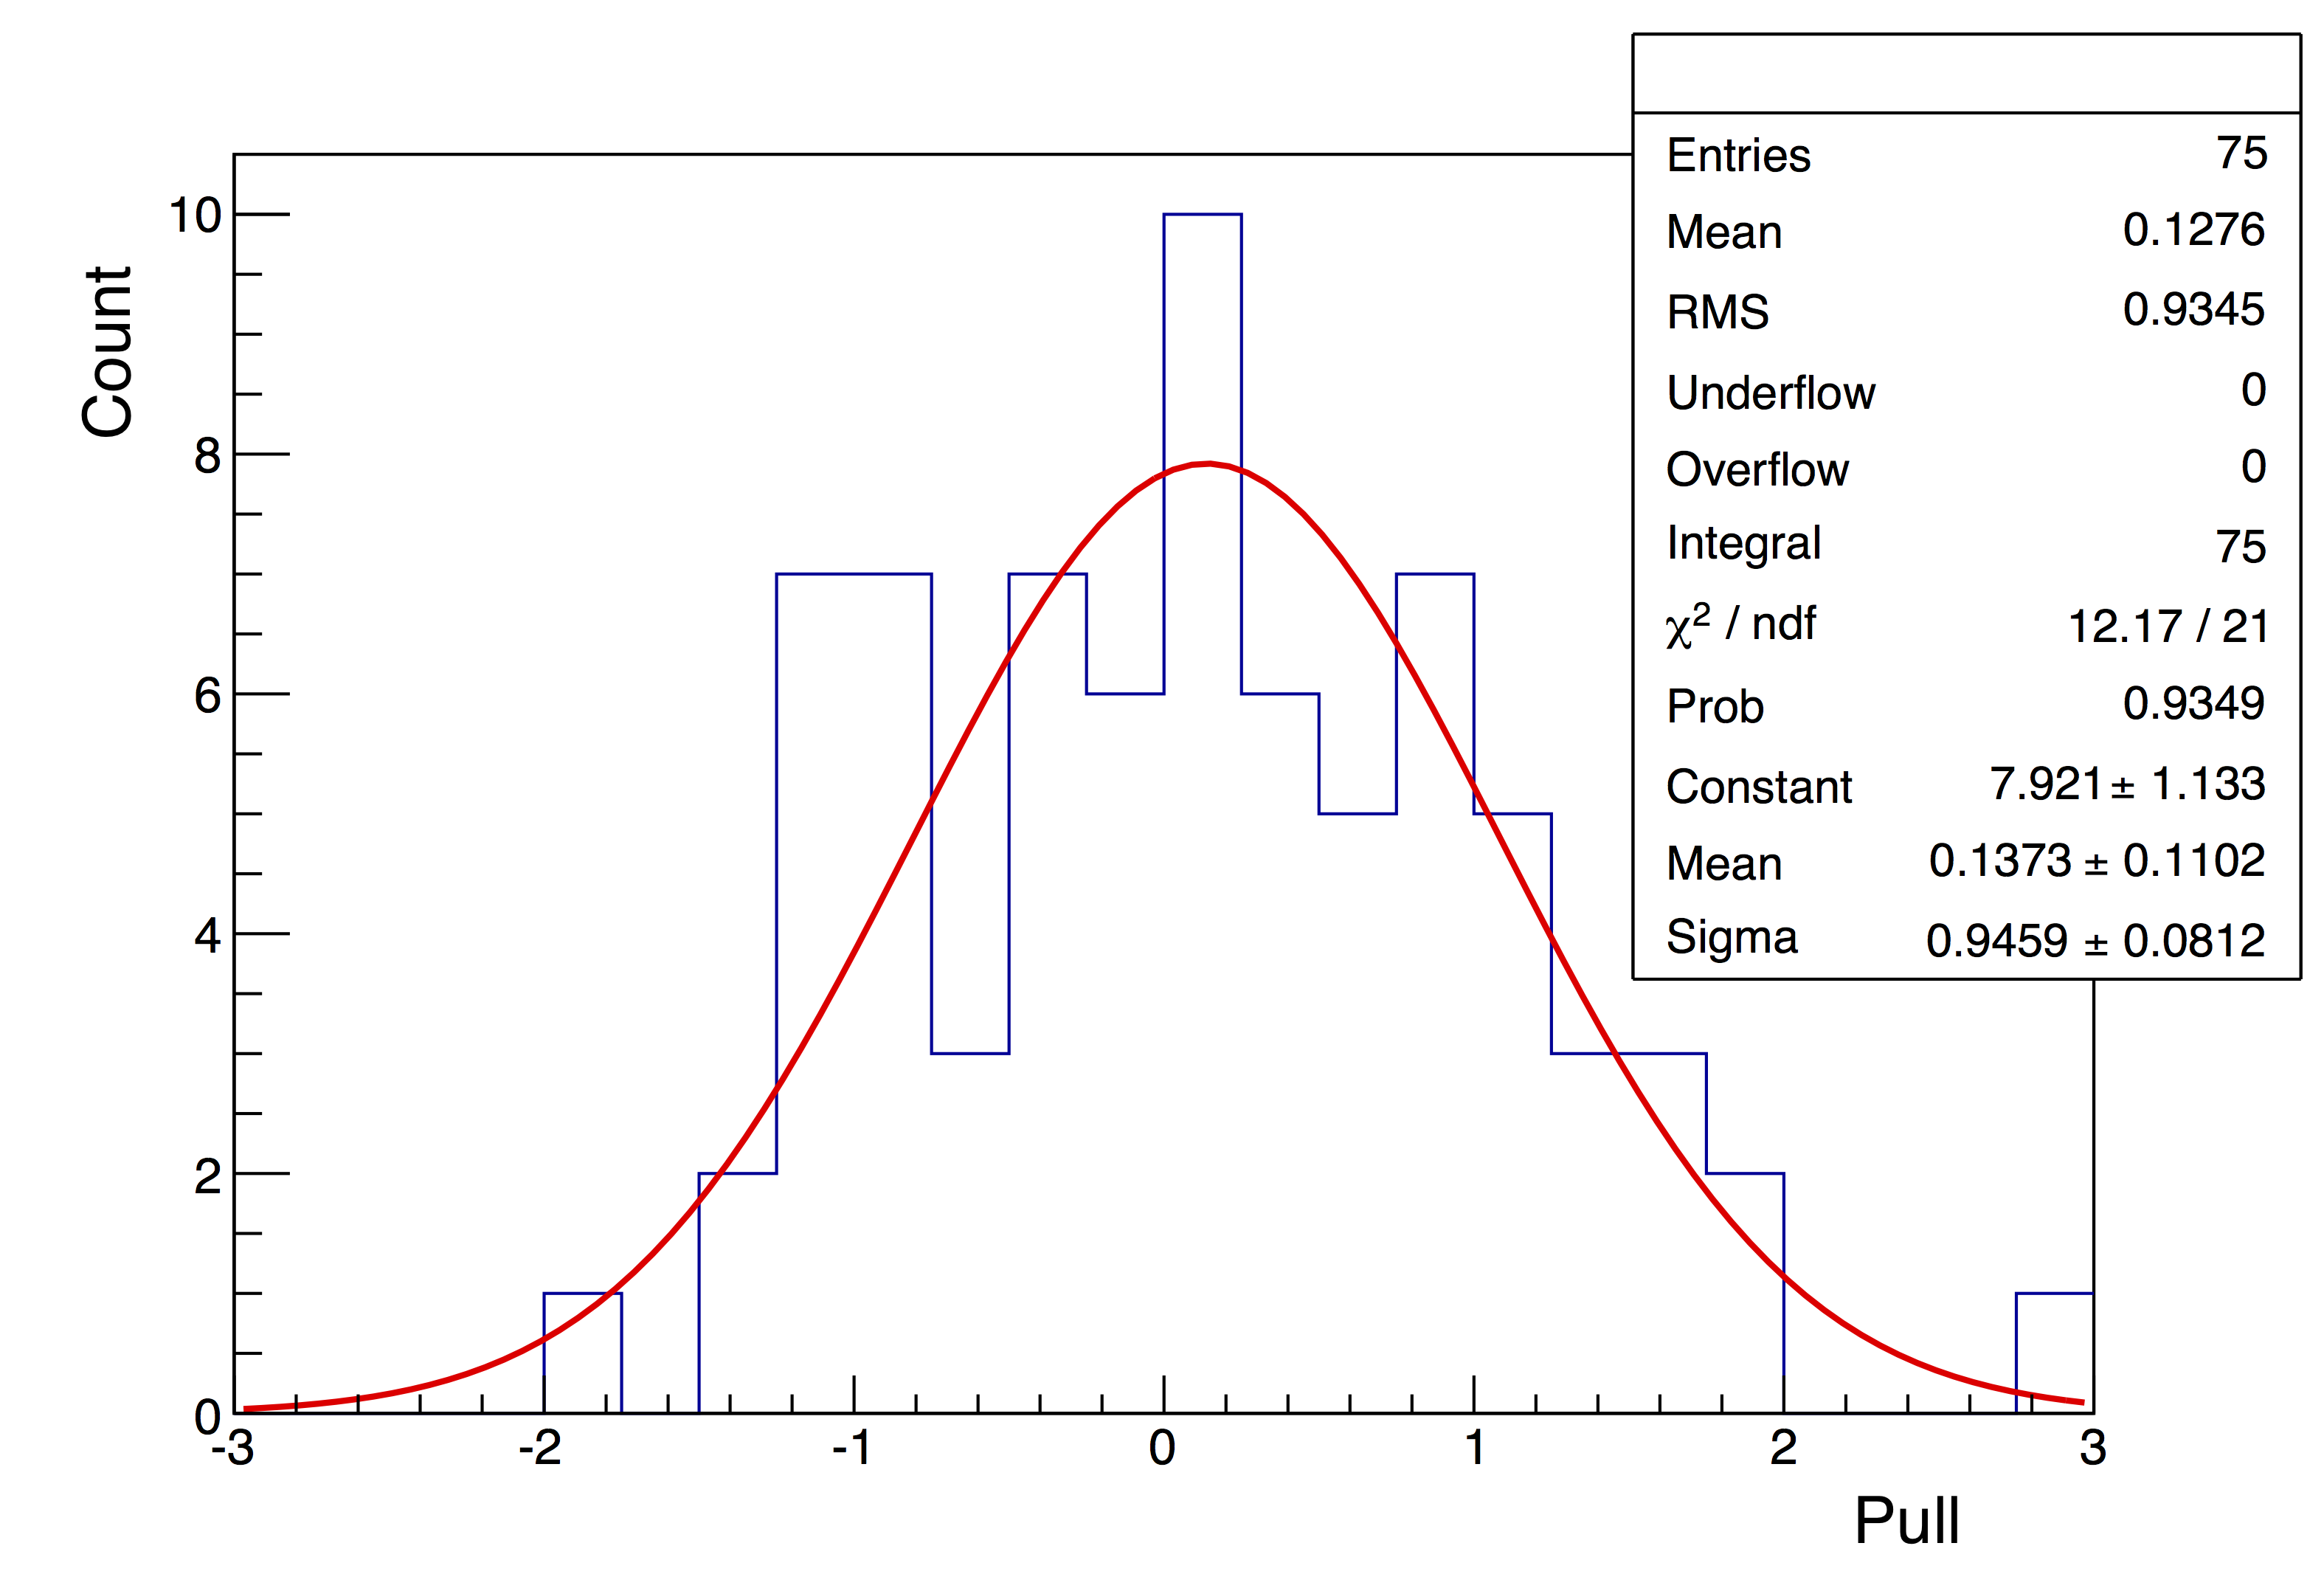
\includegraphics[width=\textwidth]{Figs/results/v0/pulls/pull_per_bin_img.png}
    \caption{}
    \label{fig:pull_distro}
  \end{subfigure}
  \begin{subfigure}[b]{0.46\textwidth}
    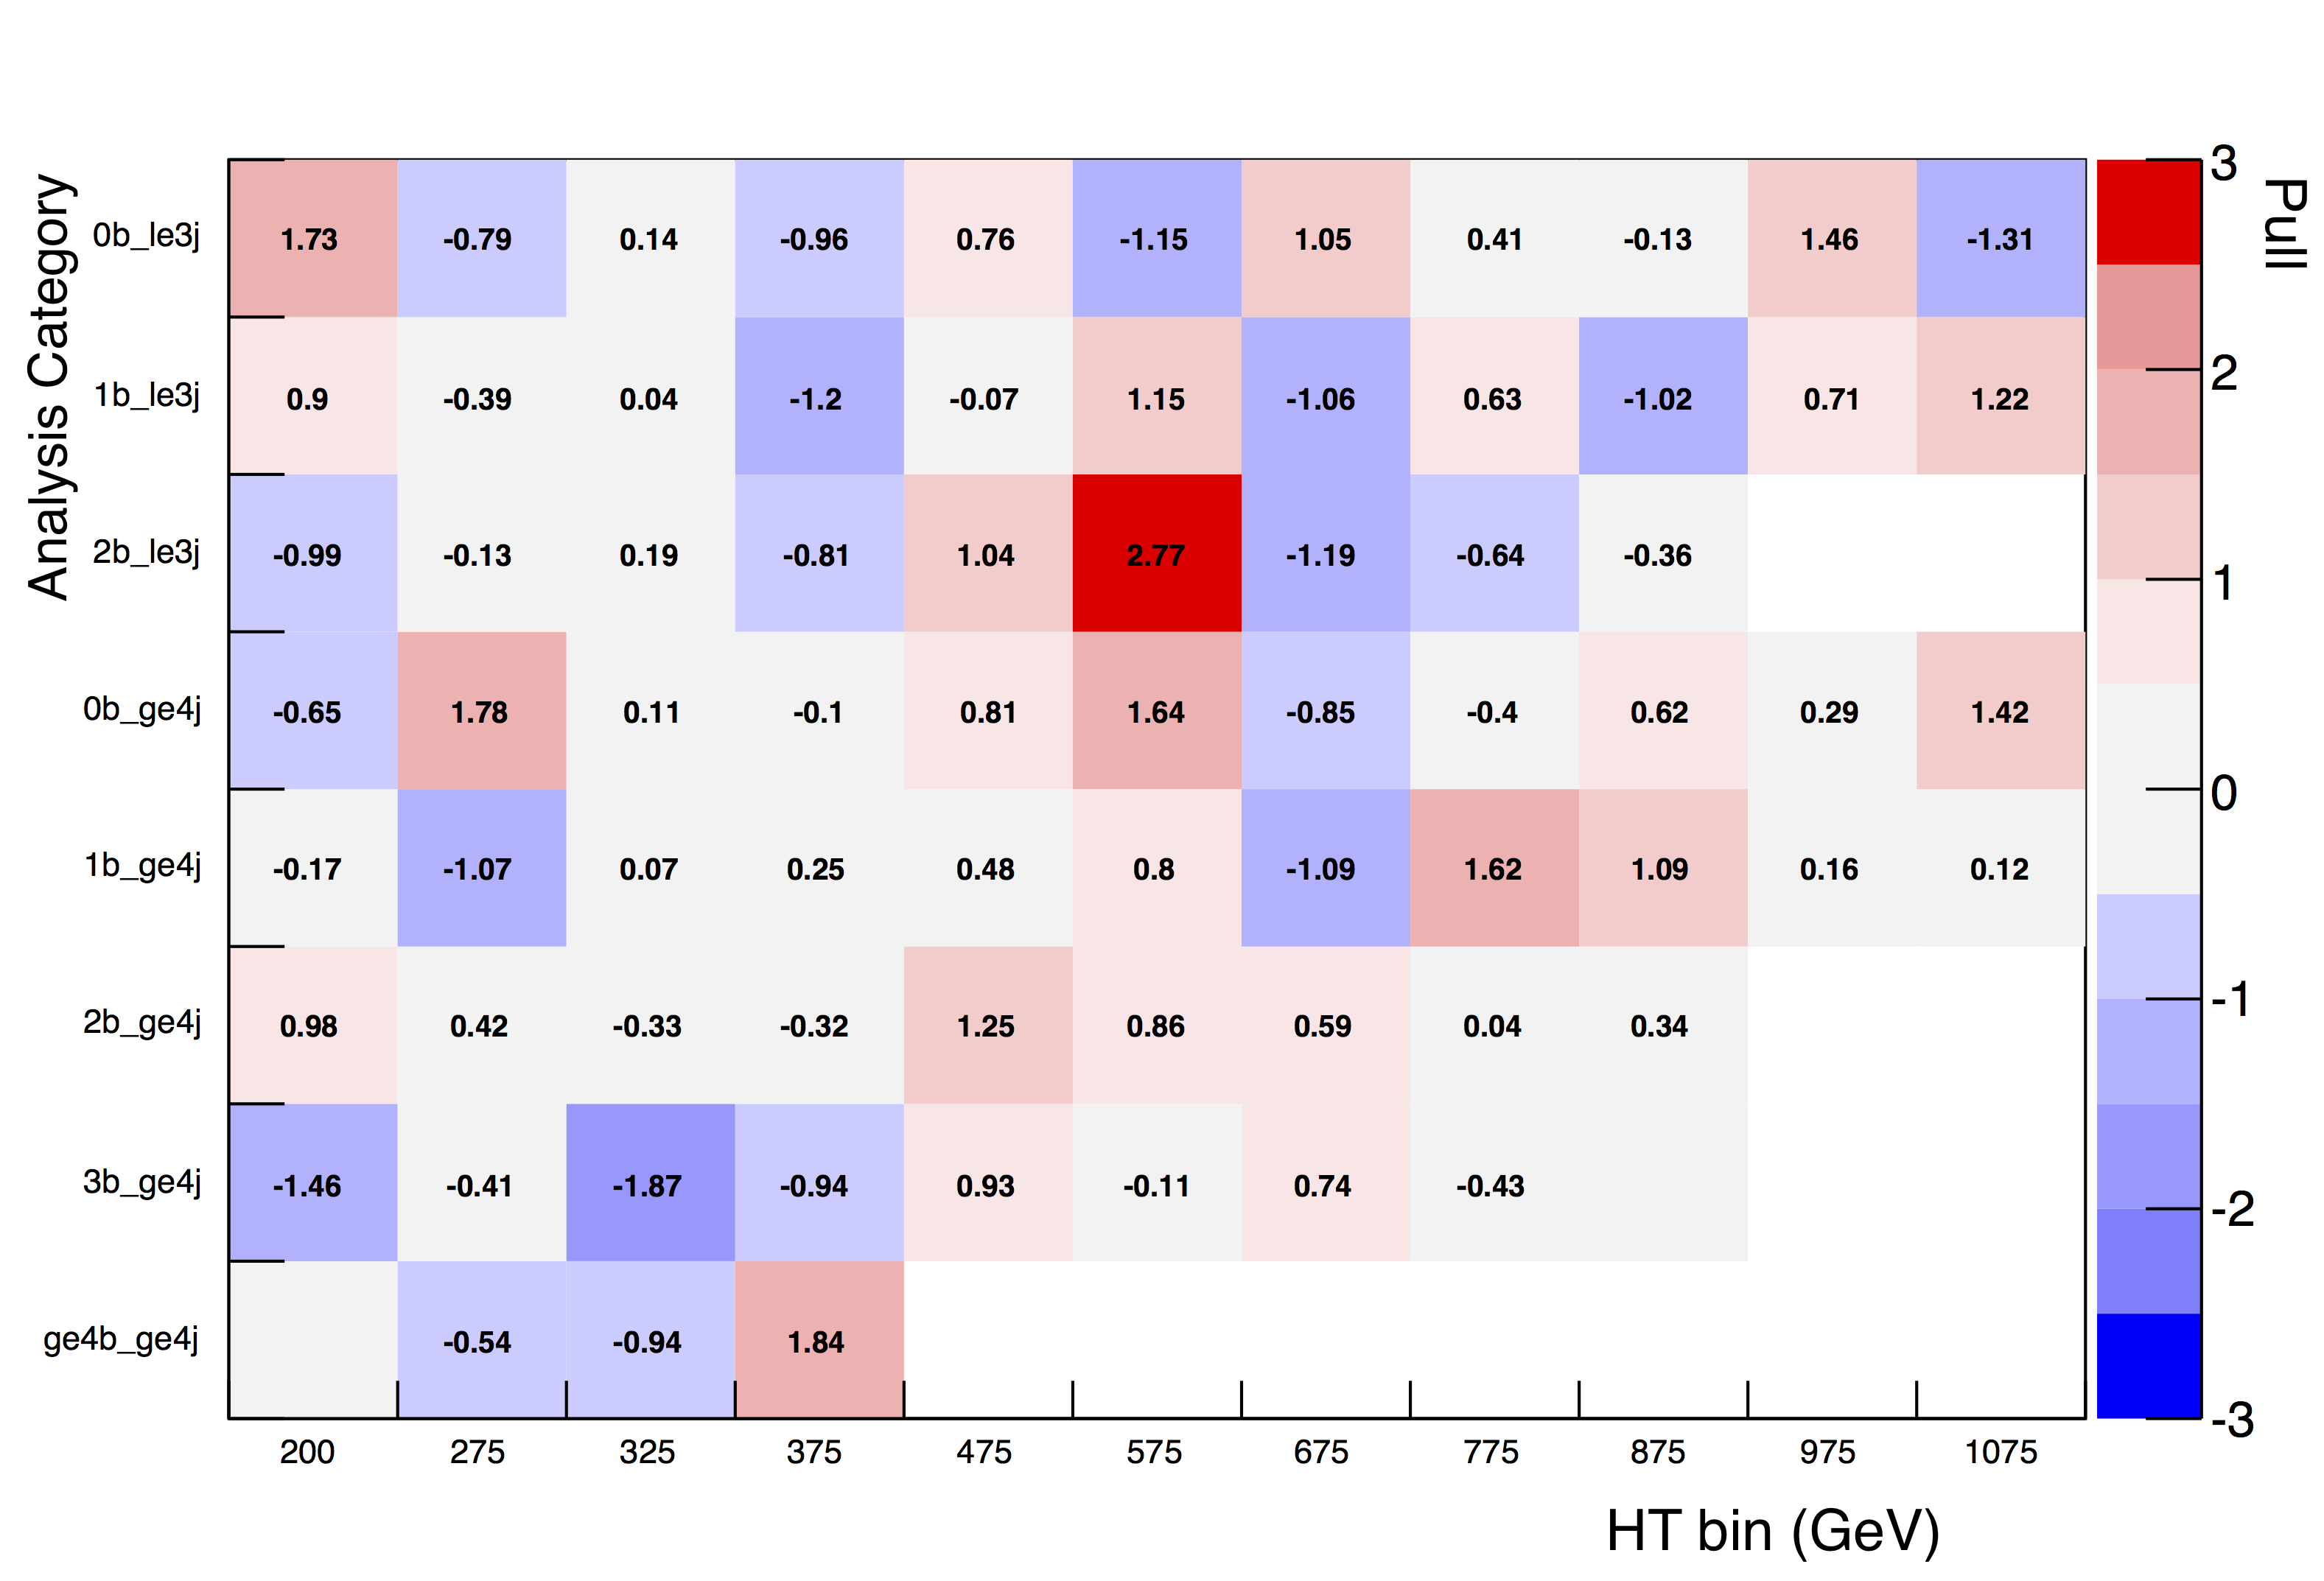
\includegraphics[width=\textwidth]{Figs/results/v0/pulls/chris_latest2_2_img.png}
    \caption{}
    \label{fig:french_flag}
  \end{subfigure}\\
  \begin{subfigure}[b]{0.46\textwidth}
    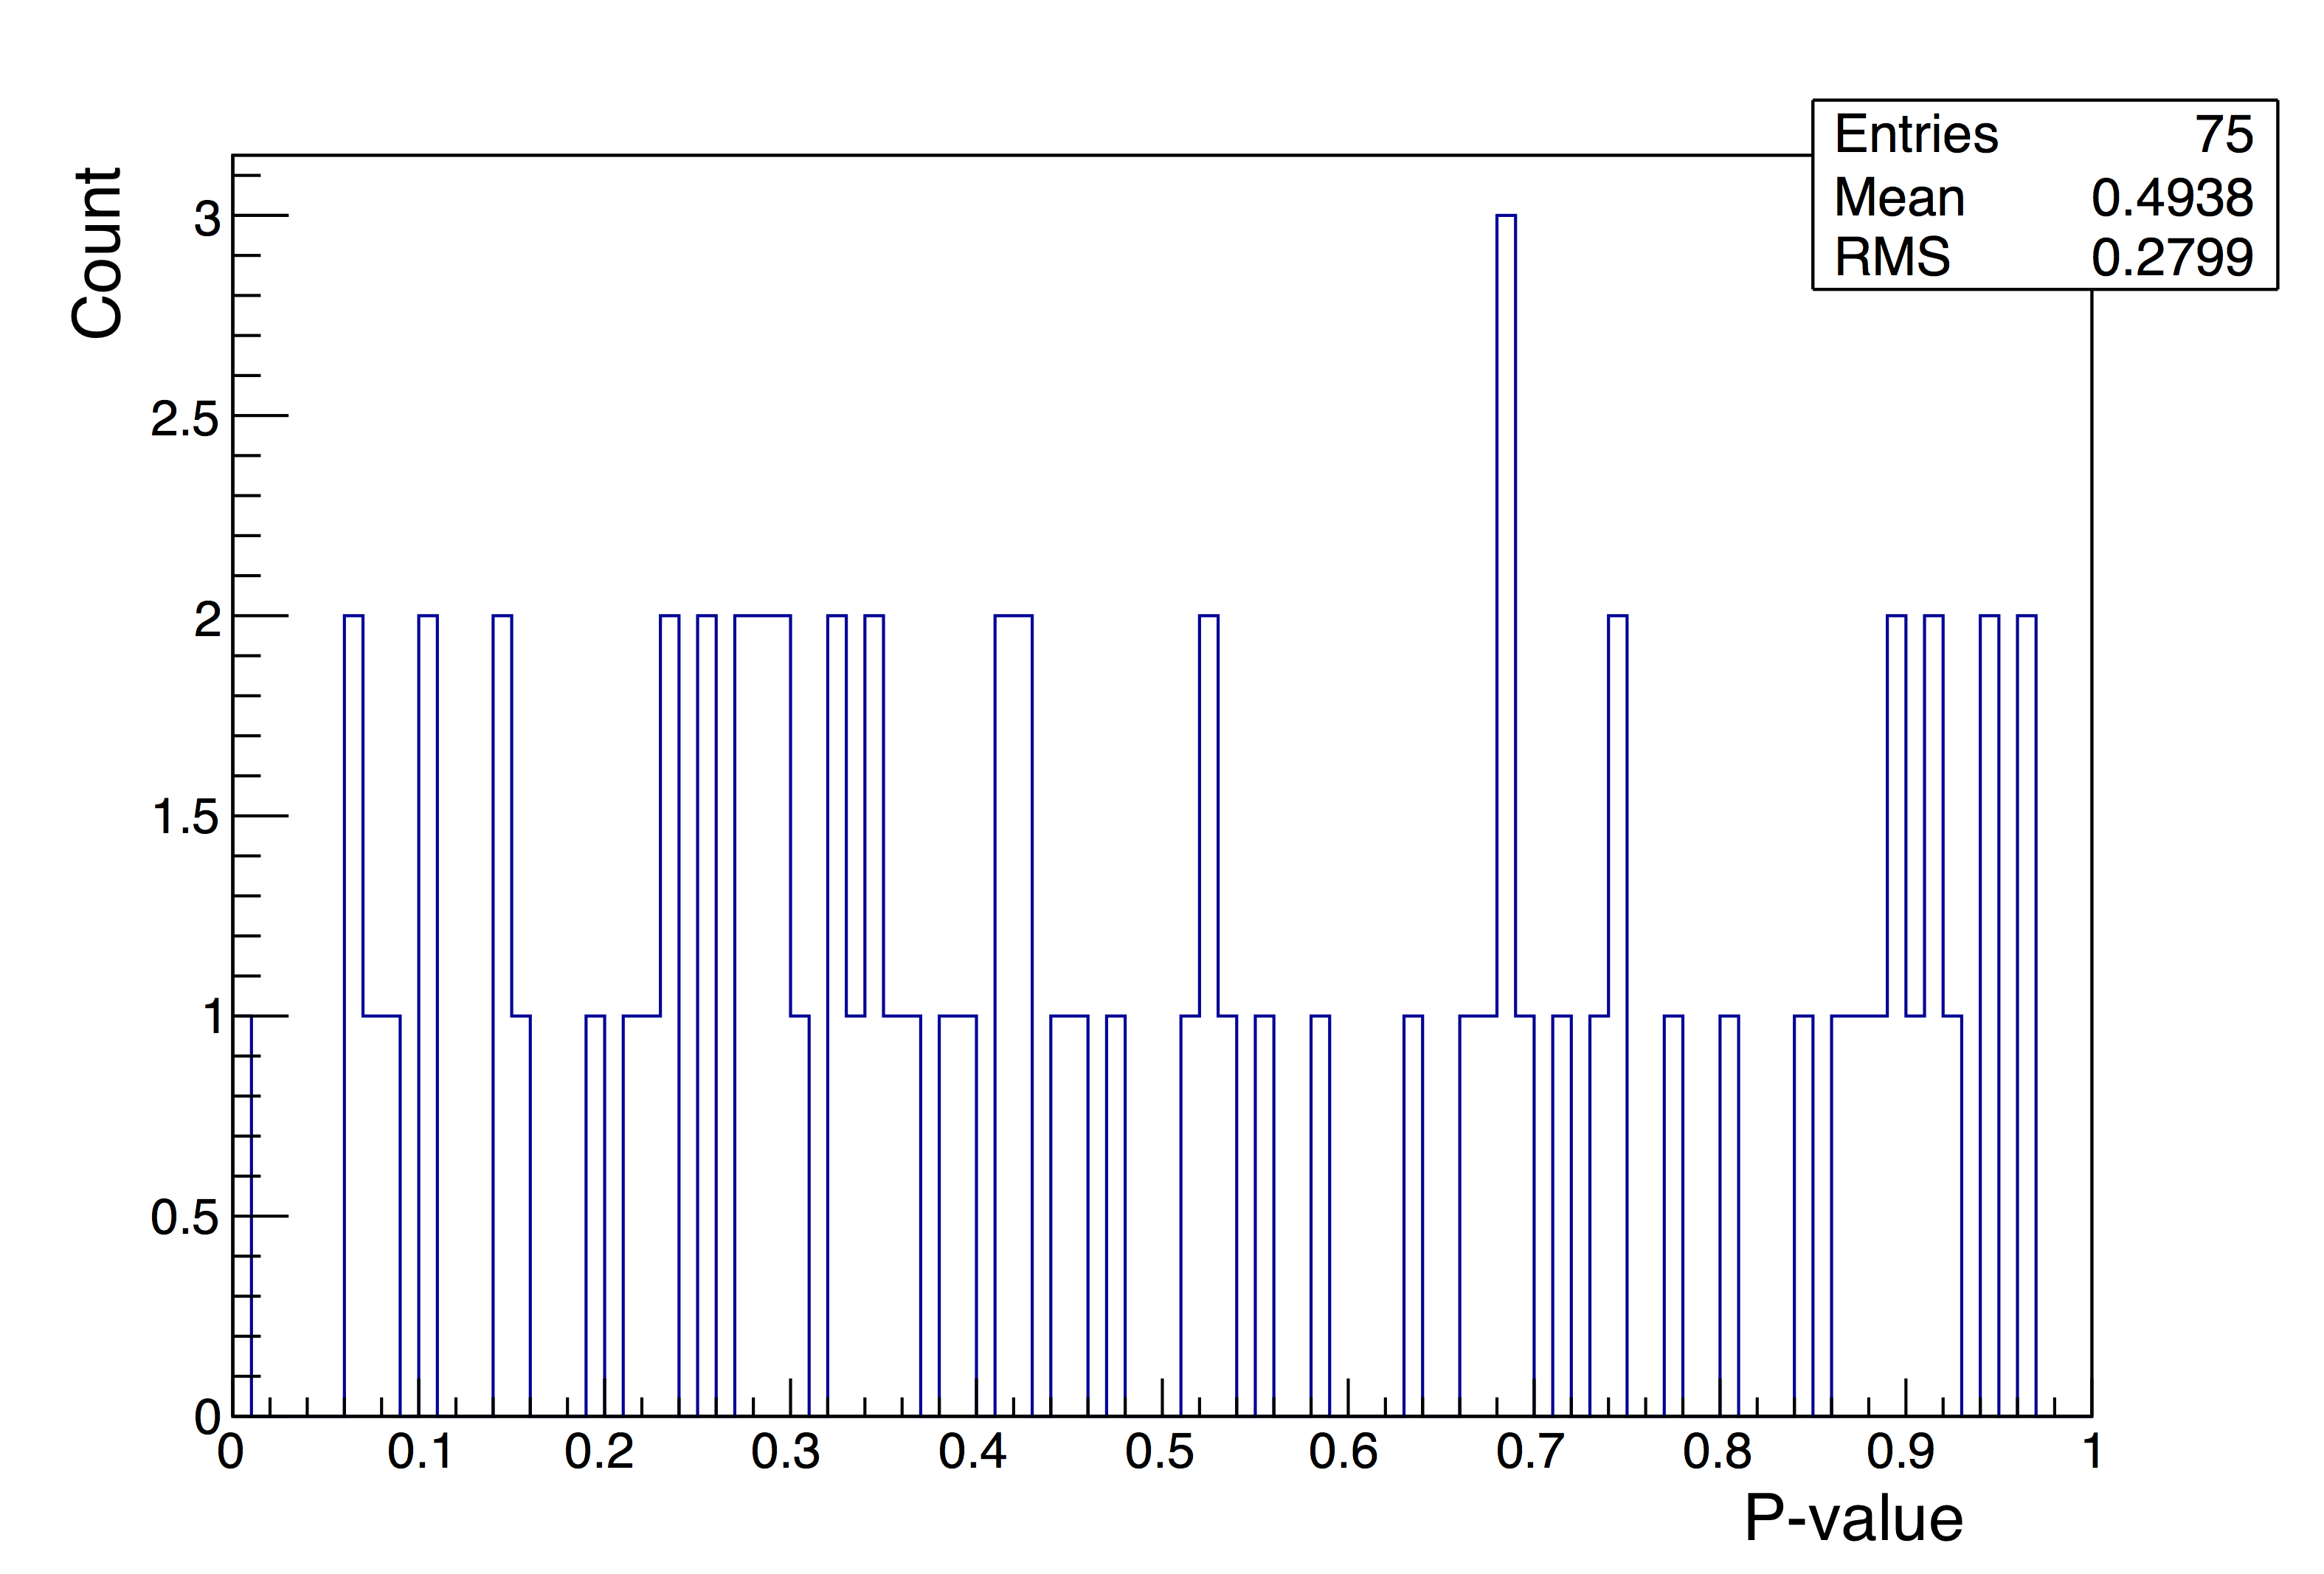
\includegraphics[width=\textwidth]{Figs/results/v0/pulls/pvalue_per_bin_img.png}
    \caption{}
    \label{fig:pvalue_distro}
  \end{subfigure}
  \begin{subfigure}[b]{0.46\textwidth}
    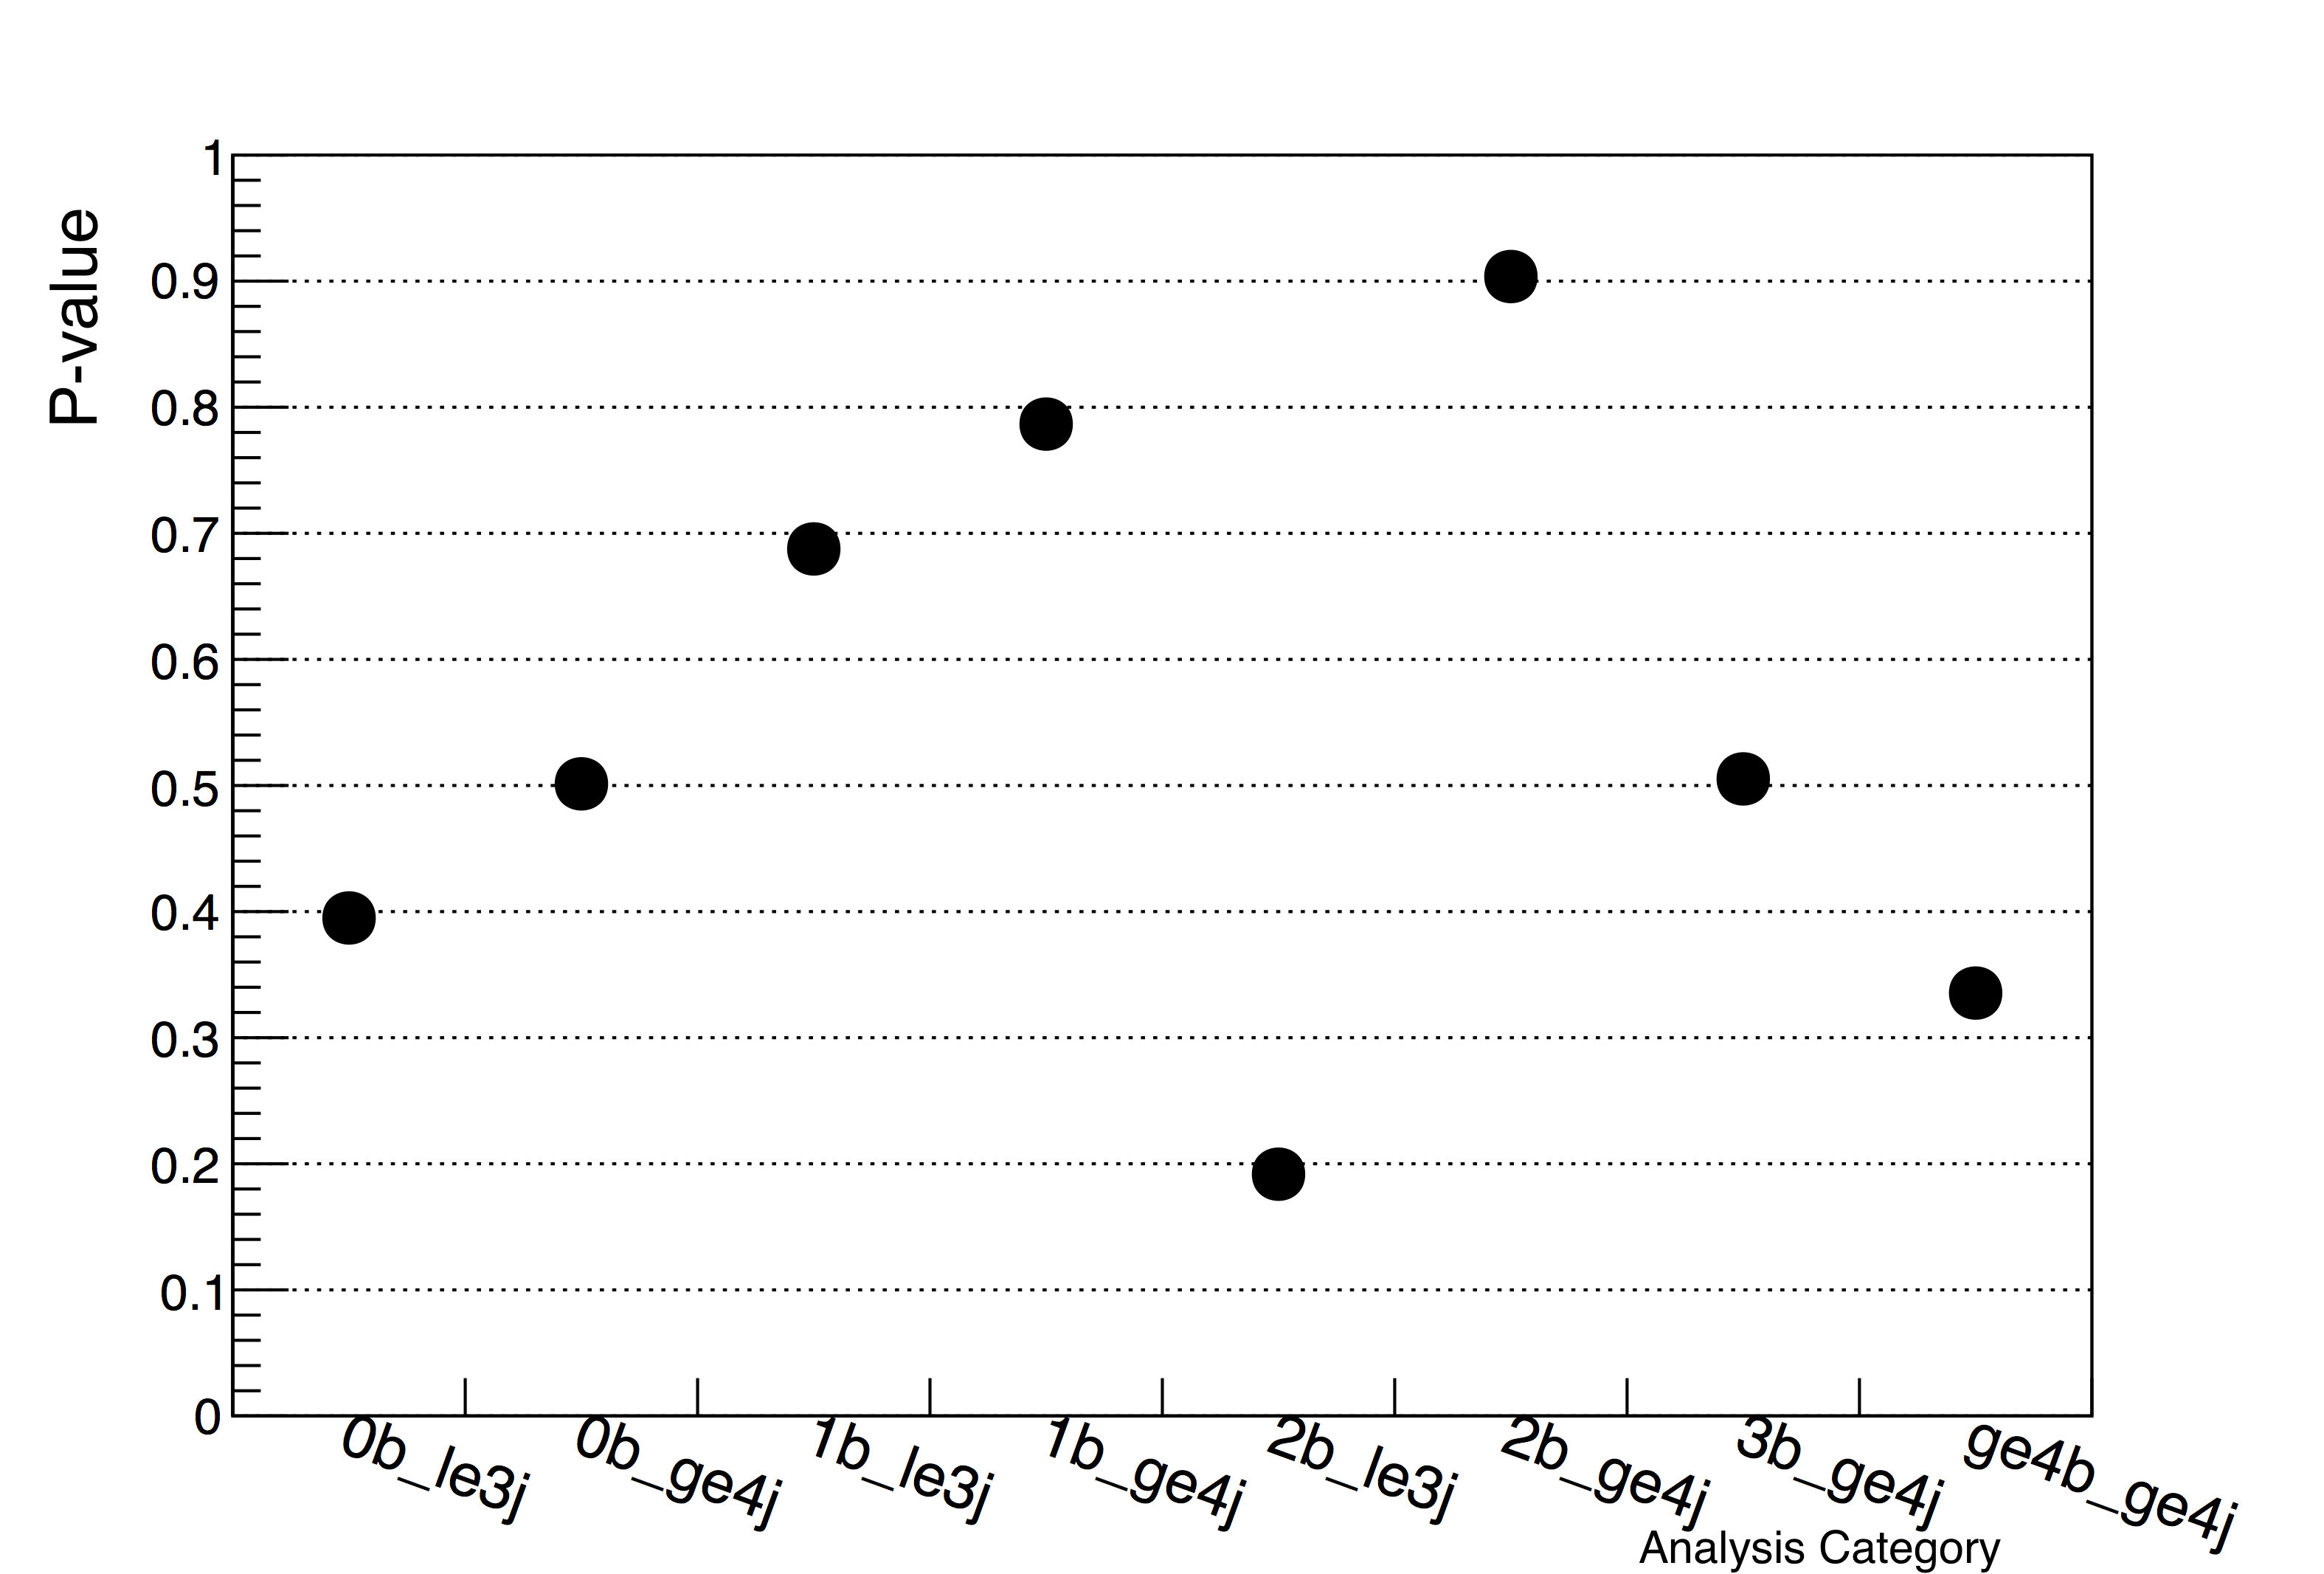
\includegraphics[width=\textwidth]{Figs/results/v0/pulls/pvalue_vs_cat_img.png}
    \caption{}
    \label{fig:pvalue_per_cat}
  \end{subfigure}
  \caption{Pulls for each analysis bin shown as a 1D distribution
  (Figure~\ref{fig:pull_distro}) and as a function of the \HT bin and analysis
  category (\nj, \nb) (Figure~\ref{fig:french_flag}). P-values for every
  analysis bin shown as a 1D distribution (Figure~\ref{fig:pvalue_distro}) and
  for each analysis category, for an inclusive \HT range
  (Figure~\ref{fig:pvalue_per_cat}).}
  \label{fig:pull_analysis}
\end{figure}

% Pulls are defined as the deviation of the observation away from the background
% prediction, divided by it's error, while a p-value is
% calculated as the
% quantile of the distribution of maximised likelihood values for an ensemble of
% pseudo-experiments.

The goodness-of-fit of the SM-only hypothesis is determined using a profile-likelihood method
taken from~\cite{Cowan:358560}.
The observed maximised likelihood value, $L^{data}_{max}$, is used as a
PDF to generate
pseudo-experiments for which the likelihood is again maximised giving the 
value $L_{max}$. These
values are entered into a histogram from which the $L^{data}_{max}$ quantile is taken, 
interpreted as the p-value and further converted into a observed significance,
or pull.
The p-values and pulls are summarised for various different analysis categories and individual
\HT bins in the plots shown in Figure~\ref{fig:pull_analysis}.

The 1D distribution of the
pulls is shown in Figure~\ref{fig:pull_distro}, with a Gaussian fit (red)
indicating good Gaussian behaviour, with mean and sigma values statistically
compatible with 0 and 1, respectively. Furthermore, the distribution of
these pulls as a function of the \HT bin and
the analysis category (\nb, \nj) is shown in Figure~\ref{fig:french_flag} to be
randomly distributed, with no apparent pattern to a given region.

The distribution of p-values for every bin of \HT and analysis category can be
seen in Figure~\ref{fig:pvalue_distro} to be uniformly distributed between 0
and 1. The same information is shown in Figure~\ref{fig:pvalue_per_cat} when a
single p-value is calculated for an entire \HT range, for each analysis
category, where the lowest value is 0.19.

% These tests indicate no significant excesses, and that all observations are
% compatible with statistical fluctuations.



%%%%%%%%%%%%%%%%%%%%%%%%%%%%%%%%%%%
% GREEN BAND PLOTS
%%%%%%%%%%%%%%%%%%%%%%%%%%%%%%%%%%%

\clearpage
\begin{figure}[h!]
  \centering
  \begin{subfigure}[b]{0.48\textwidth}
    \begin{overpic}[width=\textwidth]{Figs/results/v0/greenBand/single_plots/hadronic_0b_le3j.pdf}
      \put(44,62){
\includegraphics[width=1.5cm]{Figs/results/v0/ht_white_cmsprelim_cover.png}}
    \end{overpic}
    \caption{Hadronic region (linear scale)}
  \end{subfigure}
  \vspace{0.7cm}\begin{subfigure}[b]{0.48\textwidth}
    \begin{overpic}[width=\textwidth]{Figs/results/v0/greenBand/single_plots/hadronic_0b_le3j_logy.pdf}
      \put(44,62){
\includegraphics[width=1.5cm]{Figs/results/v0/ht_white_cmsprelim_cover.png}}
    \end{overpic}
    \caption{Hadronic region (logarithmic scale)}
  \end{subfigure}
  \begin{subfigure}[b]{0.48\textwidth}
    \begin{overpic}[width=\textwidth]{Figs/results/v0/greenBand/single_plots/muon_0b_le3j_logy.pdf}
      \put(12,20){
\includegraphics[width=1.5cm]{Figs/results/v0/ht_white_cmsprelim_cover.png}}
    \end{overpic}
    \caption{\mj region}
  \end{subfigure}
  \begin{subfigure}[b]{0.48\textwidth}
    \begin{overpic}[width=\textwidth]{Figs/results/v0/greenBand/single_plots/mumu_0b_le3j_logy.pdf}
      \put(44,63){
\includegraphics[width=1.5cm]{Figs/results/v0/ht_white_cmsprelim_cover.png}}
    \end{overpic}
    \caption{\mmj region}
  \end{subfigure}\\
  \vspace{0.7cm}\begin{subfigure}[b]{0.48\textwidth}
    \begin{overpic}[width=\textwidth]{Figs/results/v0/greenBand/single_plots/photon_0b_le3j_logy.pdf}
      \put(44,63){
\includegraphics[width=1.5cm]{Figs/results/v0/ht_white_cmsprelim_cover.png}}
    \end{overpic}
    \caption{\gj region}
  \end{subfigure}
  \caption{Observations in data for the signal and control
  regions of the analysis, compared to the result of the full likelihood model
  simultaneous fit, when the hadronic data observations are not considered. The
  plots shown are for the \njlow, $\nb = 0$ analysis category.}
  \label{fig:green_fits_0b_le3j}
\end{figure}

\clearpage
\begin{figure}[h!]
  \centering
  \begin{subfigure}[b]{0.48\textwidth}
    \begin{overpic}[width=\textwidth]{Figs/results/v0/greenBand/single_plots/hadronic_1b_le3j.pdf}
      \put(44,62){
\includegraphics[width=1.5cm]{Figs/results/v0/ht_white_cmsprelim_cover.png}}
    \end{overpic}
    \caption{Hadronic region (linear scale)}
  \end{subfigure}
  \vspace{0.7cm}\begin{subfigure}[b]{0.48\textwidth}
    \begin{overpic}[width=\textwidth]{Figs/results/v0/greenBand/single_plots/hadronic_1b_le3j_logy.pdf}
      \put(44,62){
\includegraphics[width=1.5cm]{Figs/results/v0/ht_white_cmsprelim_cover.png}}
    \end{overpic}
    \caption{Hadronic region (logarithmic scale)}
  \end{subfigure}
  \begin{subfigure}[b]{0.48\textwidth}
    \begin{overpic}[width=\textwidth]{Figs/results/v0/greenBand/single_plots/muon_1b_le3j_logy.pdf}
      \put(12,20){
\includegraphics[width=1.5cm]{Figs/results/v0/ht_white_cmsprelim_cover.png}}
    \end{overpic}
    \caption{\mj region}
  \end{subfigure}
  \begin{subfigure}[b]{0.48\textwidth}
    \begin{overpic}[width=\textwidth]{Figs/results/v0/greenBand/single_plots/mumu_1b_le3j_logy.pdf}
      \put(44,63){
\includegraphics[width=1.5cm]{Figs/results/v0/ht_white_cmsprelim_cover.png}}
    \end{overpic}
    \caption{\mmj region}
  \end{subfigure}\\
  \vspace{0.7cm}\begin{subfigure}[b]{0.48\textwidth}
    \begin{overpic}[width=\textwidth]{Figs/results/v0/greenBand/single_plots/photon_1b_le3j_logy.pdf}
      \put(44,63){
\includegraphics[width=1.5cm]{Figs/results/v0/ht_white_cmsprelim_cover.png}}
    \end{overpic}
    \caption{\gj region}
  \end{subfigure}
  \caption{Observations in data for the signal and control
  regions of the analysis, compared to the result of the full likelihood model
  simultaneous fit, when the hadronic data observations are not considered. The
  plots shown are for the \njlow, $\nb = 1$ analysis category.}
  \label{fig:green_fits_1b_le3j}
\end{figure}

\clearpage
\begin{figure}[h!]
  \centering
  \begin{subfigure}[b]{0.48\textwidth}
    \begin{overpic}[width=\textwidth]{Figs/results/v0/greenBand/single_plots/hadronic_2b_le3j.pdf}
      \put(44,62){
\includegraphics[width=1.5cm]{Figs/results/v0/ht_white_cmsprelim_cover.png}}
    \end{overpic}
    \caption{Hadronic region (linear scale)}
  \end{subfigure}
  \vspace{0.7cm}\begin{subfigure}[b]{0.48\textwidth}
    \begin{overpic}[width=\textwidth]{Figs/results/v0/greenBand/single_plots/hadronic_2b_le3j_logy.pdf}
      \put(44,62){
\includegraphics[width=1.5cm]{Figs/results/v0/ht_white_cmsprelim_cover.png}}
    \end{overpic}
    \caption{Hadronic region (logarithmic scale)}
  \end{subfigure}
  \begin{subfigure}[b]{0.48\textwidth}
    \begin{overpic}[width=\textwidth]{Figs/results/v0/greenBand/single_plots/muon_2b_le3j_logy.pdf}
      \put(12,20){
\includegraphics[width=1.5cm]{Figs/results/v0/ht_white_cmsprelim_cover.png}}
    \end{overpic}
    \caption{\mj region}
  \end{subfigure}
  \caption{Observations in data for the signal and control
  regions of the analysis, compared to the result of the full likelihood model
  simultaneous fit, when the hadronic data observations are not considered. The
  plots shown are for the \njlow, $\nb = 2$ analysis category.}
  \label{fig:green_fits_2b_le3j}
\end{figure}

\clearpage
\begin{figure}[h!]
  \centering
  \begin{subfigure}[b]{0.48\textwidth}
    \begin{overpic}[width=\textwidth]{Figs/results/v0/greenBand/single_plots/hadronic_0b_ge4j.pdf}
      \put(44,62){
\includegraphics[width=1.5cm]{Figs/results/v0/ht_white_cmsprelim_cover.png}}
    \end{overpic}
    \caption{Hadronic region (linear scale)}
  \end{subfigure}
  \vspace{0.7cm}\begin{subfigure}[b]{0.48\textwidth}
    \begin{overpic}[width=\textwidth]{Figs/results/v0/greenBand/single_plots/hadronic_0b_ge4j_logy.pdf}
      \put(44,62){
\includegraphics[width=1.5cm]{Figs/results/v0/ht_white_cmsprelim_cover.png}}
    \end{overpic}
    \caption{Hadronic region (logarithmic scale)}
  \end{subfigure}
  \begin{subfigure}[b]{0.48\textwidth}
    \begin{overpic}[width=\textwidth]{Figs/results/v0/greenBand/single_plots/muon_0b_ge4j_logy.pdf}
      \put(12,20){
\includegraphics[width=1.5cm]{Figs/results/v0/ht_white_cmsprelim_cover.png}}
    \end{overpic}
    \caption{\mj region}
  \end{subfigure}
  \begin{subfigure}[b]{0.48\textwidth}
    \begin{overpic}[width=\textwidth]{Figs/results/v0/greenBand/single_plots/mumu_0b_ge4j_logy.pdf}
      \put(44,63){
\includegraphics[width=1.5cm]{Figs/results/v0/ht_white_cmsprelim_cover.png}}
    \end{overpic}
    \caption{\mmj region}
  \end{subfigure}\\
  \vspace{0.7cm}\begin{subfigure}[b]{0.48\textwidth}
    \begin{overpic}[width=\textwidth]{Figs/results/v0/greenBand/single_plots/photon_0b_ge4j_logy.pdf}
      \put(44,63){
\includegraphics[width=1.5cm]{Figs/results/v0/ht_white_cmsprelim_cover.png}}
    \end{overpic}
    \caption{\gj region}
  \end{subfigure}
  \caption{Observations in data for the signal and control
  regions of the analysis, compared to the result of the full likelihood model
  simultaneous fit, when the hadronic data observations are not considered. The
  plots shown are for the \njhigh, $\nb = 0$ analysis category.}
  \label{fig:green_fits_0b_ge4j}
\end{figure}

\clearpage
\begin{figure}[h!]
  \centering
  \begin{subfigure}[b]{0.48\textwidth}
    \begin{overpic}[width=\textwidth]{Figs/results/v0/greenBand/single_plots/hadronic_1b_ge4j.pdf}
      \put(44,62){
\includegraphics[width=1.5cm]{Figs/results/v0/ht_white_cmsprelim_cover.png}}
    \end{overpic}
    \caption{Hadronic region (linear scale)}
  \end{subfigure}
  \vspace{0.7cm}\begin{subfigure}[b]{0.48\textwidth}
    \begin{overpic}[width=\textwidth]{Figs/results/v0/greenBand/single_plots/hadronic_1b_ge4j_logy.pdf}
      \put(44,62){
\includegraphics[width=1.5cm]{Figs/results/v0/ht_white_cmsprelim_cover.png}}
    \end{overpic}
    \caption{Hadronic region (logarithmic scale)}
  \end{subfigure}
  \begin{subfigure}[b]{0.48\textwidth}
    \begin{overpic}[width=\textwidth]{Figs/results/v0/greenBand/single_plots/muon_1b_ge4j_logy.pdf}
      \put(12,20){
\includegraphics[width=1.5cm]{Figs/results/v0/ht_white_cmsprelim_cover.png}}
    \end{overpic}
    \caption{\mj region}
  \end{subfigure}
  \begin{subfigure}[b]{0.48\textwidth}
    \begin{overpic}[width=\textwidth]{Figs/results/v0/greenBand/single_plots/mumu_1b_ge4j_logy.pdf}
      \put(44,63){
\includegraphics[width=1.5cm]{Figs/results/v0/ht_white_cmsprelim_cover.png}}
    \end{overpic}
    \caption{\mmj region}
  \end{subfigure}\\
  \vspace{0.7cm}\begin{subfigure}[b]{0.48\textwidth}
    \begin{overpic}[width=\textwidth]{Figs/results/v0/greenBand/single_plots/photon_1b_ge4j_logy.pdf}
      \put(44,63){
\includegraphics[width=1.5cm]{Figs/results/v0/ht_white_cmsprelim_cover.png}}
    \end{overpic}
    \caption{\gj region}
  \end{subfigure}
  \caption{Observations in data for the signal and control
  regions of the analysis, compared to the result of the full likelihood model
  simultaneous fit, when the hadronic data observations are not considered. The
  plots shown are for the \njhigh, $\nb = 1$ analysis category.}
  \label{fig:green_fits_1b_ge4j}
\end{figure}

\clearpage
\begin{figure}[h!]
  \centering
  \begin{subfigure}[b]{0.48\textwidth}
    \begin{overpic}[width=\textwidth]{Figs/results/v0/greenBand/single_plots/hadronic_2b_ge4j.pdf}
      \put(44,62){
\includegraphics[width=1.5cm]{Figs/results/v0/ht_white_cmsprelim_cover.png}}
    \end{overpic}
    \caption{Hadronic region (linear scale)}
  \end{subfigure}
  \vspace{0.7cm}\begin{subfigure}[b]{0.48\textwidth}
    \begin{overpic}[width=\textwidth]{Figs/results/v0/greenBand/single_plots/hadronic_2b_ge4j_logy.pdf}
      \put(44,62){
\includegraphics[width=1.5cm]{Figs/results/v0/ht_white_cmsprelim_cover.png}}
    \end{overpic}
    \caption{Hadronic region (logarithmic scale)}
  \end{subfigure}
  \begin{subfigure}[b]{0.48\textwidth}
    \begin{overpic}[width=\textwidth]{Figs/results/v0/greenBand/single_plots/muon_2b_ge4j_logy.pdf}
      \put(12,20){
\includegraphics[width=1.5cm]{Figs/results/v0/ht_white_cmsprelim_cover.png}}
    \end{overpic}
    \caption{\mj region}
  \end{subfigure}
  \caption{Observations in data for the signal and control
  regions of the analysis, compared to the result of the full likelihood model
  simultaneous fit, when the hadronic data observations are not considered. The
  plots shown are for the \njhigh, $\nb = 2$ analysis category.}
  \label{fig:green_fits_2b_ge4j}
\end{figure}


\clearpage
\begin{figure}[h!]
  \centering
  \begin{subfigure}[b]{0.48\textwidth}
    \begin{overpic}[width=\textwidth]{Figs/results/v0/greenBand/single_plots/hadronic_3b_ge4j.pdf}
      \put(44,62){
\includegraphics[width=1.5cm]{Figs/results/v0/ht_white_cmsprelim_cover.png}}
    \end{overpic}
    \caption{Hadronic region (linear scale)}
  \end{subfigure}
  \vspace{0.7cm}\begin{subfigure}[b]{0.48\textwidth}
    \begin{overpic}[width=\textwidth]{Figs/results/v0/greenBand/single_plots/hadronic_3b_ge4j_logy.pdf}
      \put(44,62){
\includegraphics[width=1.5cm]{Figs/results/v0/ht_white_cmsprelim_cover.png}}
    \end{overpic}
    \caption{Hadronic region (logarithmic scale)}
  \end{subfigure}
  \begin{subfigure}[b]{0.48\textwidth}
    \begin{overpic}[width=\textwidth]{Figs/results/v0/greenBand/single_plots/muon_3b_ge4j_logy.pdf}
      \put(12,20){
\includegraphics[width=1.5cm]{Figs/results/v0/ht_white_cmsprelim_cover.png}}
    \end{overpic}
    \caption{\mj region}
  \end{subfigure}
  \caption{Observations in data for the signal and control
  regions of the analysis, compared to the result of the full likelihood model
  simultaneous fit, when the hadronic data observations are not considered. The
  plots shown are for the \njhigh, $\nb = 3$ analysis category.}
  \label{fig:green_fits_3b_ge4j}
\end{figure}

\clearpage
\begin{figure}[h!]
  \centering
  \begin{subfigure}[b]{0.48\textwidth}
    \begin{overpic}[width=\textwidth]{Figs/results/v0/greenBand/single_plots/hadronic_ge4b_ge4j.pdf}
      \put(44,62){
\includegraphics[width=1.5cm]{Figs/results/v0/ht_white_cmsprelim_cover.png}}
    \end{overpic}
    \caption{Hadronic region (linear scale)}
  \end{subfigure}
  \vspace{0.7cm}\begin{subfigure}[b]{0.48\textwidth}
    \begin{overpic}[width=\textwidth]{Figs/results/v0/greenBand/single_plots/hadronic_ge4b_ge4j_logy.pdf}
      \put(44,62){
\includegraphics[width=1.5cm]{Figs/results/v0/ht_white_cmsprelim_cover.png}}
    \end{overpic}
    \caption{Hadronic region (logarithmic scale)}
  \end{subfigure}
  \begin{subfigure}[b]{0.48\textwidth}
    \begin{overpic}[width=\textwidth]{Figs/results/v0/greenBand/single_plots/muon_ge4b_ge4j_logy.pdf}
      \put(44,63){
\includegraphics[width=1.5cm]{Figs/results/v0/ht_white_cmsprelim_cover.png}}
    \end{overpic}
    \caption{\mj region}
  \end{subfigure}
  \caption{Observations in data for the signal and control
  regions of the analysis, compared to the result of the full likelihood model
  simultaneous fit, when the hadronic data observations are not considered. The
  plots shown are for the \njhigh, $\nb \geq 4$ analysis category.}
  \label{fig:green_fits_ge4b_ge4j}
\end{figure}

%%%%%%%%%%%%%%%%%%%%%%%%%%%%%%%%%%%
% BLUE BAND PLOTS
%%%%%%%%%%%%%%%%%%%%%%%%%%%%%%%%%%%

\clearpage
\begin{figure}[h!]
  \centering
  \begin{subfigure}[b]{0.48\textwidth}
    \begin{overpic}[width=\textwidth]{Figs/results/v0/blueBand/single_plots/hadronic_0b_le3j.pdf}
      \put(44,62){
\includegraphics[width=1.5cm]{Figs/results/v0/ht_white_cmsprelim_cover.png}}
    \end{overpic}
    \caption{Hadronic region (linear scale)}
  \end{subfigure}
  \vspace{0.7cm}\begin{subfigure}[b]{0.48\textwidth}
    \begin{overpic}[width=\textwidth]{Figs/results/v0/blueBand/single_plots/hadronic_0b_le3j_logy.pdf}
      \put(44,62){
\includegraphics[width=1.5cm]{Figs/results/v0/ht_white_cmsprelim_cover.png}}
    \end{overpic}
    \caption{Hadronic region (logarithmic scale)}
  \end{subfigure}
  \begin{subfigure}[b]{0.48\textwidth}
    \begin{overpic}[width=\textwidth]{Figs/results/v0/blueBand/single_plots/muon_0b_le3j_logy.pdf}
      \put(12,20){
\includegraphics[width=1.5cm]{Figs/results/v0/ht_white_cmsprelim_cover.png}}
    \end{overpic}
    \caption{\mj region}
  \end{subfigure}
  \begin{subfigure}[b]{0.48\textwidth}
    \begin{overpic}[width=\textwidth]{Figs/results/v0/blueBand/single_plots/mumu_0b_le3j_logy.pdf}
      \put(44,63){
\includegraphics[width=1.5cm]{Figs/results/v0/ht_white_cmsprelim_cover.png}}
    \end{overpic}
    \caption{\mmj region}
  \end{subfigure}\\
  \vspace{0.7cm}\begin{subfigure}[b]{0.48\textwidth}
    \begin{overpic}[width=\textwidth]{Figs/results/v0/blueBand/single_plots/photon_0b_le3j_logy.pdf}
      \put(44,63){
\includegraphics[width=1.5cm]{Figs/results/v0/ht_white_cmsprelim_cover.png}}
    \end{overpic}
    \caption{\gj region}
  \end{subfigure}
  \caption{Observations in data for the signal and control
  regions of the analysis, compared to the result of the full likelihood model
  simultaneous fit. The
  plots shown are for the \njlow, $\nb = 0$ analysis category.}
  \label{fig:blue_fits_0b_le3j}
\end{figure}

\clearpage
\begin{figure}[h!]
  \centering
  \begin{subfigure}[b]{0.48\textwidth}
    \begin{overpic}[width=\textwidth]{Figs/results/v0/blueBand/single_plots/hadronic_1b_le3j.pdf}
      \put(44,62){
\includegraphics[width=1.5cm]{Figs/results/v0/ht_white_cmsprelim_cover.png}}
    \end{overpic}
    \caption{Hadronic region (linear scale)}
  \end{subfigure}
  \vspace{0.7cm}\begin{subfigure}[b]{0.48\textwidth}
    \begin{overpic}[width=\textwidth]{Figs/results/v0/blueBand/single_plots/hadronic_1b_le3j_logy.pdf}
      \put(44,62){
\includegraphics[width=1.5cm]{Figs/results/v0/ht_white_cmsprelim_cover.png}}
    \end{overpic}
    \caption{Hadronic region (logarithmic scale)}
  \end{subfigure}
  \begin{subfigure}[b]{0.48\textwidth}
    \begin{overpic}[width=\textwidth]{Figs/results/v0/blueBand/single_plots/muon_1b_le3j_logy.pdf}
      \put(12,20){
\includegraphics[width=1.5cm]{Figs/results/v0/ht_white_cmsprelim_cover.png}}
    \end{overpic}
    \caption{\mj region}
  \end{subfigure}
  \begin{subfigure}[b]{0.48\textwidth}
    \begin{overpic}[width=\textwidth]{Figs/results/v0/blueBand/single_plots/mumu_1b_le3j_logy.pdf}
      \put(44,63){
\includegraphics[width=1.5cm]{Figs/results/v0/ht_white_cmsprelim_cover.png}}
    \end{overpic}
    \caption{\mmj region}
  \end{subfigure}\\
  \vspace{0.7cm}\begin{subfigure}[b]{0.48\textwidth}
    \begin{overpic}[width=\textwidth]{Figs/results/v0/blueBand/single_plots/photon_1b_le3j_logy.pdf}
      \put(44,63){
\includegraphics[width=1.5cm]{Figs/results/v0/ht_white_cmsprelim_cover.png}}
    \end{overpic}
    \caption{\gj region}
  \end{subfigure}
  \caption{Observations in data for the signal and control
  regions of the analysis, compared to the result of the full likelihood model
  simultaneous fit. The
  plots shown are for the \njlow, $\nb = 1$ analysis category.}
  \label{fig:blue_fits_1b_le3j}
\end{figure}

\clearpage
\begin{figure}[h!]
  \centering
  \begin{subfigure}[b]{0.48\textwidth}
    \begin{overpic}[width=\textwidth]{Figs/results/v0/blueBand/single_plots/hadronic_2b_le3j.pdf}
      \put(44,62){
\includegraphics[width=1.5cm]{Figs/results/v0/ht_white_cmsprelim_cover.png}}
    \end{overpic}
    \caption{Hadronic region (linear scale)}
  \end{subfigure}
  \vspace{0.7cm}\begin{subfigure}[b]{0.48\textwidth}
    \begin{overpic}[width=\textwidth]{Figs/results/v0/blueBand/single_plots/hadronic_2b_le3j_logy.pdf}
      \put(44,62){
\includegraphics[width=1.5cm]{Figs/results/v0/ht_white_cmsprelim_cover.png}}
    \end{overpic}
    \caption{Hadronic region (logarithmic scale)}
  \end{subfigure}
  \begin{subfigure}[b]{0.48\textwidth}
    \begin{overpic}[width=\textwidth]{Figs/results/v0/blueBand/single_plots/muon_2b_le3j_logy.pdf}
      \put(12,20){
\includegraphics[width=1.5cm]{Figs/results/v0/ht_white_cmsprelim_cover.png}}
    \end{overpic}
    \caption{\mj region}
  \end{subfigure}
  \caption{Observations in data for the signal and control
  regions of the analysis, compared to the result of the full likelihood model
  simultaneous fit. The
  plots shown are for the \njlow, $\nb = 2$ analysis category.}
  \label{fig:blue_fits_2b_le3j}
\end{figure}

\clearpage
\begin{figure}[h!]
  \centering
  \begin{subfigure}[b]{0.48\textwidth}
    \begin{overpic}[width=\textwidth]{Figs/results/v0/blueBand/single_plots/hadronic_0b_ge4j.pdf}
      \put(44,62){
\includegraphics[width=1.5cm]{Figs/results/v0/ht_white_cmsprelim_cover.png}}
    \end{overpic}
    \caption{Hadronic region (linear scale)}
  \end{subfigure}
  \vspace{0.7cm}\begin{subfigure}[b]{0.48\textwidth}
    \begin{overpic}[width=\textwidth]{Figs/results/v0/blueBand/single_plots/hadronic_0b_ge4j_logy.pdf}
      \put(44,62){\includegraphics[width=1.5cm]{Figs/results/v0/ht_white_cmsprelim_cover.png}}
    \end{overpic}
    \caption{Hadronic region (logarithmic scale)}
  \end{subfigure}
  \begin{subfigure}[b]{0.48\textwidth}
    \begin{overpic}[width=\textwidth]{Figs/results/v0/blueBand/single_plots/muon_0b_ge4j_logy.pdf}
      \put(12,20){\includegraphics[width=1.5cm]{Figs/results/v0/ht_white_cmsprelim_cover.png}}
    \end{overpic}
    \caption{\mj region}
  \end{subfigure}
  \begin{subfigure}[b]{0.48\textwidth}
    \begin{overpic}[width=\textwidth]{Figs/results/v0/blueBand/single_plots/mumu_0b_ge4j_logy.pdf}
      \put(44,63){\includegraphics[width=1.5cm]{Figs/results/v0/ht_white_cmsprelim_cover.png}}
    \end{overpic}
    \caption{\mmj region}
  \end{subfigure}\\
  \vspace{0.7cm}\begin{subfigure}[b]{0.48\textwidth}
    \begin{overpic}[width=\textwidth]{Figs/results/v0/blueBand/single_plots/photon_0b_ge4j_logy.pdf}
      \put(44,63){\includegraphics[width=1.5cm]{Figs/results/v0/ht_white_cmsprelim_cover.png}}
    \end{overpic}
    \caption{\gj region}
  \end{subfigure}
  \caption{Observations in data for the signal and control
  regions of the analysis, compared to the result of the full likelihood model
  simultaneous fit. The
  plots shown are for the \njhigh, $\nb = 0$ analysis category.}
  \label{fig:blue_fits_0b_ge4j}
\end{figure}

\clearpage
\begin{figure}[h!]
  \centering
  \begin{subfigure}[b]{0.48\textwidth}
    \begin{overpic}[width=\textwidth]{Figs/results/v0/blueBand/single_plots/hadronic_1b_ge4j.pdf}
      \put(44,62){\includegraphics[width=1.5cm]{Figs/results/v0/ht_white_cmsprelim_cover.png}}
    \end{overpic}
    \caption{Hadronic region (linear scale)}
  \end{subfigure}
  \vspace{0.7cm}\begin{subfigure}[b]{0.48\textwidth}
    \begin{overpic}[width=\textwidth]{Figs/results/v0/blueBand/single_plots/hadronic_1b_ge4j_logy.pdf}
      \put(44,62){\includegraphics[width=1.5cm]{Figs/results/v0/ht_white_cmsprelim_cover.png}}
    \end{overpic}
    \caption{Hadronic region (logarithmic scale)}
  \end{subfigure}
  \begin{subfigure}[b]{0.48\textwidth}
    \begin{overpic}[width=\textwidth]{Figs/results/v0/blueBand/single_plots/muon_1b_ge4j_logy.pdf}
      \put(12,20){\includegraphics[width=1.5cm]{Figs/results/v0/ht_white_cmsprelim_cover.png}}
    \end{overpic}
    \caption{\mj region}
  \end{subfigure}
  \begin{subfigure}[b]{0.48\textwidth}
    \begin{overpic}[width=\textwidth]{Figs/results/v0/blueBand/single_plots/mumu_1b_ge4j_logy.pdf}
      \put(44,63){\includegraphics[width=1.5cm]{Figs/results/v0/ht_white_cmsprelim_cover.png}}
    \end{overpic}
    \caption{\mmj region}
  \end{subfigure}\\
  \vspace{0.7cm}\begin{subfigure}[b]{0.48\textwidth}
    \begin{overpic}[width=\textwidth]{Figs/results/v0/blueBand/single_plots/photon_1b_ge4j_logy.pdf}
      \put(44,63){\includegraphics[width=1.5cm]{Figs/results/v0/ht_white_cmsprelim_cover.png}}
    \end{overpic}
    \caption{\gj region}
  \end{subfigure}
  \caption{Observations in data for the signal and control
  regions of the analysis, compared to the result of the full likelihood model
  simultaneous fit. The
  plots shown are for the \njhigh, $\nb = 1$ analysis category.}
  \label{fig:blue_fits_1b_ge4j}
\end{figure}

\clearpage
\begin{figure}[h!]
  \centering
  \begin{subfigure}[b]{0.48\textwidth}
    \begin{overpic}[width=\textwidth]{Figs/results/v0/blueBand/single_plots/hadronic_2b_ge4j.pdf}
      \put(44,62){\includegraphics[width=1.5cm]{Figs/results/v0/ht_white_cmsprelim_cover.png}}
    \end{overpic}
    \caption{Hadronic region (linear scale)}
  \end{subfigure}
  \vspace{0.7cm}\begin{subfigure}[b]{0.48\textwidth}
    \begin{overpic}[width=\textwidth]{Figs/results/v0/blueBand/single_plots/hadronic_2b_ge4j_logy.pdf}
      \put(44,62){\includegraphics[width=1.5cm]{Figs/results/v0/ht_white_cmsprelim_cover.png}}
    \end{overpic}
    \caption{Hadronic region (logarithmic scale)}
  \end{subfigure}
  \begin{subfigure}[b]{0.48\textwidth}
    \begin{overpic}[width=\textwidth]{Figs/results/v0/blueBand/single_plots/muon_2b_ge4j_logy.pdf}
      \put(12,20){\includegraphics[width=1.5cm]{Figs/results/v0/ht_white_cmsprelim_cover.png}}
    \end{overpic}
    \caption{\mj region}
  \end{subfigure}
  \caption{Observations in data for the signal and control
  regions of the analysis, compared to the result of the full likelihood model
  simultaneous fit. The
  plots shown are for the \njhigh, $\nb = 2$ analysis category.}
  \label{fig:blue_fits_2b_ge4j}
\end{figure}


\clearpage
\begin{figure}[h!]
  \centering
  \begin{subfigure}[b]{0.48\textwidth}
    \begin{overpic}[width=\textwidth]{Figs/results/v0/blueBand/single_plots/hadronic_3b_ge4j.pdf}
      \put(44,62){\includegraphics[width=1.5cm]{Figs/results/v0/ht_white_cmsprelim_cover.png}}
    \end{overpic}
    \caption{Hadronic region (linear scale)}
  \end{subfigure}
  \vspace{0.7cm}\begin{subfigure}[b]{0.48\textwidth}
    \begin{overpic}[width=\textwidth]{Figs/results/v0/blueBand/single_plots/hadronic_3b_ge4j_logy.pdf}
      \put(44,62){\includegraphics[width=1.5cm]{Figs/results/v0/ht_white_cmsprelim_cover.png}}
    \end{overpic}
    \caption{Hadronic region (logarithmic scale)}
  \end{subfigure}
  \begin{subfigure}[b]{0.48\textwidth}
    \begin{overpic}[width=\textwidth]{Figs/results/v0/blueBand/single_plots/muon_3b_ge4j_logy.pdf}
      \put(12,20){\includegraphics[width=1.5cm]{Figs/results/v0/ht_white_cmsprelim_cover.png}}
    \end{overpic}
    \caption{\mj region}
  \end{subfigure}
  \caption{Observations in data for the signal and control
  regions of the analysis, compared to the result of the full likelihood model
  simultaneous fit. The
  plots shown are for the \njhigh, $\nb = 3$ analysis category.}
  \label{fig:blue_fits_3b_ge4j}
\end{figure}

\clearpage
\begin{figure}[h!]
  \centering
  \begin{subfigure}[b]{0.48\textwidth}
    \begin{overpic}[width=\textwidth]{Figs/results/v0/blueBand/single_plots/hadronic_ge4b_ge4j.pdf}
      \put(44,62){\includegraphics[width=1.5cm]{Figs/results/v0/ht_white_cmsprelim_cover.png}}
    \end{overpic}
    \caption{Hadronic region (linear scale)}
  \end{subfigure}
  \vspace{0.7cm}\begin{subfigure}[b]{0.48\textwidth}
    \begin{overpic}[width=\textwidth]{Figs/results/v0/blueBand/single_plots/hadronic_ge4b_ge4j_logy.pdf}
      \put(44,62){\includegraphics[width=1.5cm]{Figs/results/v0/ht_white_cmsprelim_cover.png}}
    \end{overpic}
    \caption{Hadronic region (logarithmic scale)}
  \end{subfigure}
  \begin{subfigure}[b]{0.48\textwidth}
    \begin{overpic}[width=\textwidth]{Figs/results/v0/blueBand/single_plots/muon_ge4b_ge4j_logy.pdf}
      \put(44,63){\includegraphics[width=1.5cm]{Figs/results/v0/ht_white_cmsprelim_cover.png}}
    \end{overpic}
    \caption{\mj region}
  \end{subfigure}
  \caption{Observations in data for the signal and control
  regions of the analysis, compared to the result of the full likelihood model
  simultaneous fit. The
  plots shown are for the \njhigh, $\nb \geq 4$ analysis category.}
  \label{fig:blue_fits_ge4b_ge4j}
\end{figure}


\subsection{Summary}
\label{sec:results_summary}

The `a-priori' fit results described in Section~\ref{sec:results_fit_green} show the level
of agreement of the data observations in the signal region with the SM background.
This background prediction is made using the transfer factor technique described in
Chapter~\ref{ch:background}.
Good agreement is found, with only some apparent disagreement in specific \HT bins across
a small number different
analysis categories. These bins appear to be uniformly distributed throughout
the signal region, showing no particular signal-like structure. An analysis of the corresponding
pulls and p-values, described in Section~\ref{sec:results_fit}, indicates that all data
observations are statistically in agreement with the background predictions, and that
any deviations are compatible with statistical fluctuations.

Further to this, the `a-posteriori' result described in Section~\ref{sec:results_fit_blue},
allows the fit model to consider observations
in the hadronic signal region. By doing so, agreement further improves as the fit is able
to accommodate the hadronic observations without tension. This is further evidence that
data observations in the hadronic signal region are in agreement with the EWK background
predictions, and therefore the SM-only hypothesis. It is concluded then that no statistically
significant signal of BSM physics has been observed.

% a-priori predictions show the `raw' EWK prediction using only transfer factors

% this indicates a good level of agreement, with some apparent disagreement in certain
% bins of HT

% however, despite this, the fluctuations present appear to show no structure across both
% HT bins and analysis cats.

% analysis of the pvalues and pulls of this indicate that all data observations statistically
% agree with the background predictions, and any deviations are compatible with statistical
% fluctuations


% allowing the fit to consider observations in the hadronic signal region causes
% agreement to improve further, with the fit being able to accommodate the observations
% without tension.

% this is further evidence that data observations in the hadronic signal region are in agreement
% with the SM only hypothesis, and that no statistically significant signal of BSM physics has
% been observed/present.